\section{Kiến trúc và Hiện thực bộ mô phỏng DES}
\label{sec:kien-truc-hien-thuc}

\hspace{0.5cm}Nội dung tập trung làm rõ kiến trúc kỹ thuật và giải pháp hiện thực bộ mô phỏng sự kiện rời rạc (\textit{Discrete-Event Simulation -- DES}) trên nền tảng Python 3.11+ với thư viện \texttt{asyncio}, bao gồm các khía cạnh trọng tâm sau:

\begin{itemize}[leftmargin=1.5em, itemsep=2pt]
\item \textbf{Mô hình hóa hệ thống:} Vận dụng phương pháp lập trình hướng đối tượng (OOP), tham khảo các nguyên lý của mô phỏng sự kiện rời rạc phân tán (PDES) theo Richard Fujimoto, kết hợp cơ chế xử lý bất đồng bộ nhằm tổ chức và điều phối các tiến trình mô phỏng.

\item \textbf{Phạm vi và khả năng mô phỏng:} Triển khai sáu mô hình hàng đợi theo ký hiệu Kendall, từ $M/M/1$ đến $M/M/c/K$, cùng mạng hàng đợi Jackson gồm bốn trạm với cơ chế định tuyến theo xác suất.

\item \textbf{Thiết kế và kiểm chứng:} Xây dựng hệ thống theo quy trình từ thiết kế kiến trúc bằng sơ đồ UML, đặc tả các thuật toán cốt lõi đến kiểm thử và đánh giá tính đúng đắn của cơ chế xử lý sự kiện, đặc biệt là tính nhân quả trong mô phỏng.
\end{itemize}
% =========================================================================
\subsection{Thiết kế phần mềm và Mô hình hóa hướng đối tượng (UML Design)}
\label{subsec:uml-design}
% =========================================================================

\hspace{0.5cm}Kiến trúc phần mềm của bộ máy mô phỏng tuân thủ nghiêm ngặt các nguyên lý SOLID, hướng đến tính kết dính cao (\textit{High Cohesion}) và độ phụ thuộc lỏng (\textit{Loose Coupling}), được phân rã thành 4 phân hệ trụ cột gắn kết hữu cơ:

\begin{enumerate}[leftmargin=1.8em, itemsep=3.5pt]
\item \textbf{Phân hệ Điều khiển Mô phỏng Facade (\textit{Simulation Controller Subsystem}):}
\begin{itemize}[leftmargin=1.2em, itemsep=1.5pt]
\item \textit{Vai trò:} Cung cấp điểm tiếp xúc cấp cao duy nhất (\textit{Single Point of Contact}) cho ứng dụng người dùng thông qua lớp mặt tiền \texttt{Simulation} và đối tượng cấu hình \texttt{SimulationOptions} theo mô hình Hình 4 đề bài.
\item \textit{Trừu tượng hóa vận hành:} Che giấu toàn bộ độ phức tạp của việc cấp phát bộ điều phối \texttt{Dispatcher}, cấu hình hàng đợi \texttt{LadderQueue}, quản trị vòng đời và nạp tự động các tiến trình logic.
\end{itemize}

\item \textbf{Phân hệ Hạt nhân Điều phối (\textit{Simulation Engine Subsystem}):}
\begin{itemize}[leftmargin=1.2em, itemsep=1.5pt]
\item \textit{Hạt nhân điều hành trung tâm:} Quản lý vòng lặp DES, duy trì trục thời gian ảo toàn cục ($t_{\text{current}}$) và bộ đếm sự kiện qua \texttt{SequentialEventDispatcher} (tuần tự tập trung) và \texttt{DistributedEventDispatcher} (tuần tự phân vùng hàng đợi).
\item \textit{Hàng đợi ưu tiên (\texttt{BaseEventQueue}):} Thiết kế theo mẫu \textit{Strategy Pattern}, hoán đổi linh hoạt giữa cây \texttt{MinHeapPriorityQueue} ($\mathcal{O}(\log N)$) và cấu trúc phân tầng \texttt{LadderQueue} ($\bm{\mathcal{O}(1)}$ khấu hao).
\item \textit{Kiểm chứng vết:} Ghi nhận nhật ký vết thực thi (\texttt{trace\_log}) phục vụ kiểm chứng tính đơn điệu nhân quả ($t_{k+1} \ge t_k$).
\end{itemize}

\item \textbf{Phân hệ Tiến trình Logic (\textit{Logical Process Subsystem -- PDES}):}
\begin{itemize}[leftmargin=1.2em, itemsep=1.5pt]
\item \textit{Mô hình hóa PDES:} Đóng gói khép kín trạng thái nội tại (\texttt{BkSysLogicalProcessState}) và kiểm soát đồng hồ ảo cục bộ $LVT$ (\textit{Local Virtual Time}) theo nguyên lý Fujimoto.
\item \textit{Các trạm chức năng:} Kế thừa từ lớp cơ sở \texttt{BkSysLogicalProcess}, gồm trạm nguồn \texttt{SourceLP}, trạm phục vụ hợp nhất \texttt{QueueServerLP}, trạm rẽ nhánh ngẫu nhiên \texttt{BranchingServerLP}, trạm thu gom \texttt{SinkLP} và \texttt{NetworkSinkLP}.
\item \textit{Cơ chế giao tiếp:} Trao đổi dữ liệu thuần túy qua các bản tin sự kiện \texttt{Event} mang thực thể \texttt{Job}, bảo đảm nguyên tắc phi chia sẻ trạng thái (\textit{Shared-Nothing}).
\end{itemize}

\item \textbf{Phân hệ Cầu nối Bất đồng bộ \& Động cơ Coroutine (\textit{Async Integration Subsystem}):}
\begin{itemize}[leftmargin=1.2em, itemsep=1.5pt]
\item \textit{Giao tiếp phi nghẽn luồng:} Cầu nối giữa thời gian ảo gián đoạn và môi trường bất đồng bộ qua \texttt{AsyncFutureManager} (\texttt{await} phi phong tỏa).
\item \textit{Mẫu điều phối cấu trúc:} Chuẩn hóa 4 mẫu điều phối trong \texttt{AsyncTaskCoordinator}: \texttt{TaskGroup}, \texttt{gather}, \texttt{as\_completed} và \texttt{Runner}.
\item \textit{Động cơ Coroutine:} Cung cấp khung coroutine bất đồng bộ \texttt{BkSysCoLogicalProcess} và \texttt{BkSysCoEventLoop} với cơ chế \texttt{await} phi nghẽn.
\end{itemize}
\end{enumerate}


\subsubsection{Mô tả tổng quan sơ đồ cấu trúc lớp (UML Class Diagram)}
\label{subsubsec:uml-class-diagram}

\begin{figure}[H]
\centering
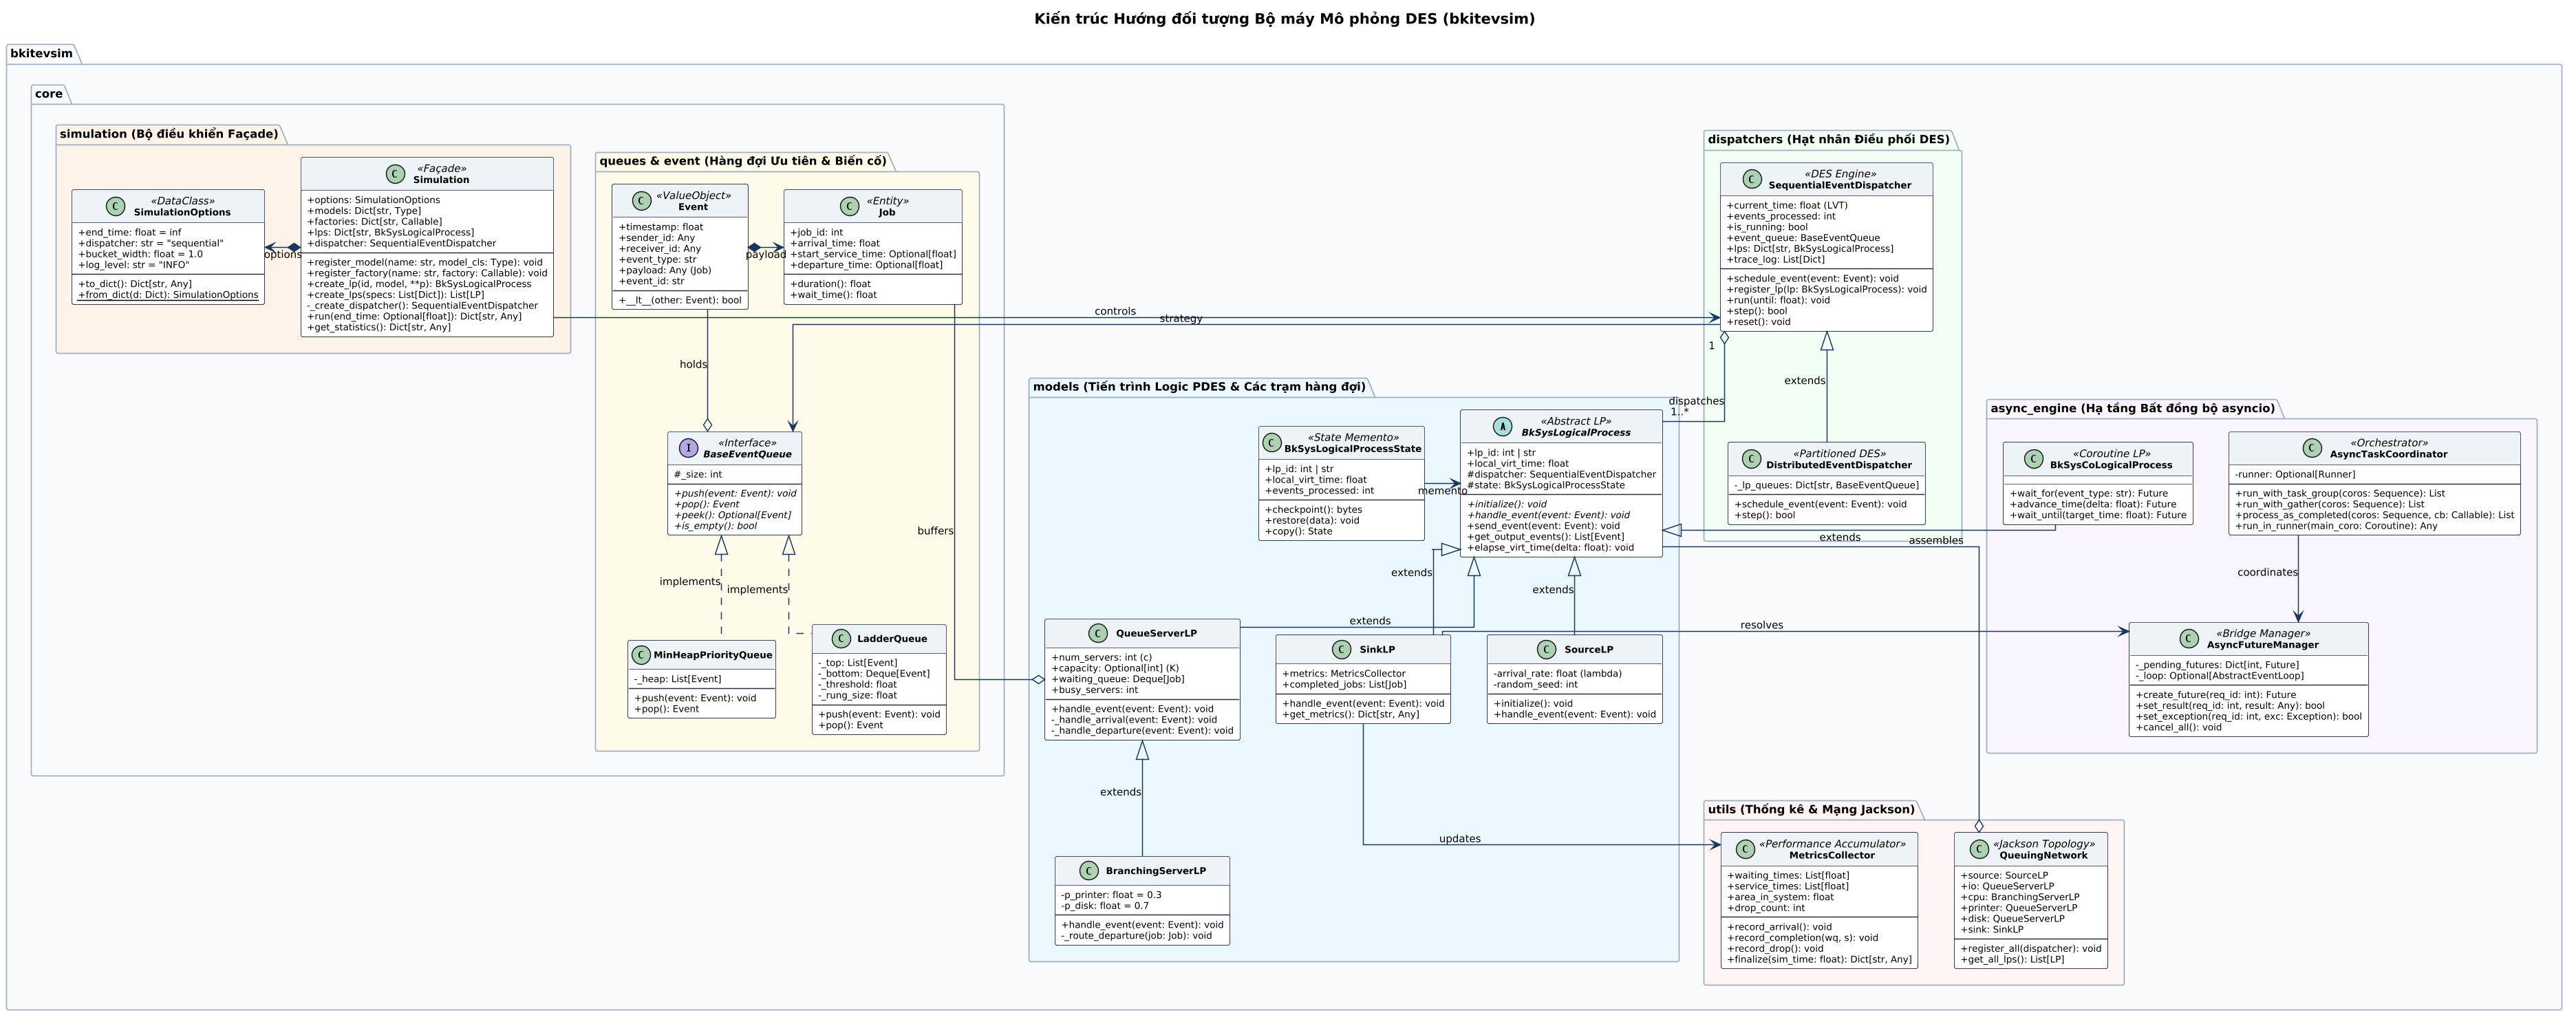
\includegraphics[width=0.98\textwidth]{image/uml_class_diagram.png}
\caption{Sơ đồ cấu trúc lớp chi tiết (UML Class Diagram) của hệ thống mô phỏng DES}
\label{fig:uml-class-diagram}
\end{figure}

\textbf{\large\hspace{0.5cm}Mô tả tổng quan sơ đồ lớp}

Sơ đồ lớp chi tiết tại Hình~\ref{fig:uml-class-diagram} đặc tả toàn diện kiến trúc hướng đối tượng của bộ máy mô phỏng sự kiện rời rạc kết hợp điều phối tác vụ bất đồng bộ (\textit{Discrete-Event Simulation with Asynchronous Task Coordination}). Hệ thống tổ chức phân tầng rõ rệt giữa bộ điều khiển Facade (\texttt{Simulation}, \texttt{SimulationOptions}), các dịch vụ điều phối sự kiện (\texttt{SequentialEventDispatcher}, \texttt{DistributedEventDispatcher}), cấu trúc hàng đợi ưu tiên (\texttt{BaseEventQueue}, \texttt{LadderQueue}), các trạm tiến trình logic PDES (\texttt{SourceLP}, \texttt{QueueServerLP}, \texttt{BranchingServerLP}, \texttt{SinkLP}) cùng hạ tầng quản lý tác vụ bất đồng bộ (\texttt{AsyncFutureManager}, \texttt{AsyncTaskCoordinator}) và thu thập số đo hiệu năng thời gian thực (\texttt{MetricsCollector}).

\textbf{\color{red}Phân hệ Điều khiển Mô phỏng Cấp cao (Simulation Controller Facade)}
\begin{itemize}[leftmargin=1.5em, itemsep=8pt]
\item \textbf{SimulationOptions}: Lớp đóng gói toàn diện các tham số cấu hình môi trường mô phỏng.

\begin{itemize}[leftmargin=1.2em, label={}, itemsep=3pt]
\item[\textendash] \textit{Thuộc tính:}
\begin{itemize}[leftmargin=1.5em, label=+, itemsep=2pt]
\item \texttt{end\_time: float} - Mốc thời gian ảo kết thúc mô phỏng (mặc định: 100.0).
\item \texttt{dispatcher: str} - Tên loại bộ điều phối (\texttt{"sequential"} hoặc \texttt{"distributed\_\allowbreak sequential"}).
\item \texttt{bucket\_width: float} - Bề rộng nấc thang $\Delta$ cho hàng đợi ưu tiên \texttt{LadderQueue}.
\item \texttt{log\_level: str} - Mức độ ghi nhật ký hệ thống (\texttt{"INFO"}, \texttt{"DEBUG"},...).
\item \texttt{log\_file: Optional[str]} - Đường dẫn tệp lưu trữ nhật ký ghi vết.
\item \texttt{stats\_file: Optional[str]} - Đường dẫn tệp xuất kết quả thống kê số liệu.
\item \texttt{verbose: bool} - Cờ bật/tắt chế độ in chi tiết tiến trình thực thi ra màn hình console.
\item \texttt{model\_params: Dict[str, Any]} - Từ điển chứa các tham số nghiệp vụ tùy biến bổ sung.
\end{itemize}

\item[\textendash] \textit{Phương thức:}
\begin{itemize}[leftmargin=1.5em, label=+, itemsep=2pt]
\item \texttt{to\_dict(): Dict[str, Any]} - Tuần tự hóa toàn bộ cấu hình sang đối tượng từ điển Python.
\item \texttt{from\_dict(data: Dict[str, Any]): SimulationOptions} - Phương thức lớp tái tạo đối tượng cấu hình từ dữ liệu từ điển/JSON.
\end{itemize}
\end{itemize}

\item \textbf{Simulation}: Lớp Facade mặt tiền điều phối cấp cao nhất, đóng vai trò là điểm chạm chính kết nối người dùng với bộ máy mô phỏng.

\begin{itemize}[leftmargin=1.2em, label={}, itemsep=3pt]
\item[\textendash] \textit{Thuộc tính:}
\begin{itemize}[leftmargin=1.5em, label=+, itemsep=2pt]
\item \texttt{options: SimulationOptions} - Đối tượng lưu trữ các cấu hình tham số vận hành.
\item \texttt{models: Dict[str, Type[BkSysLogicalProcess]]} - Danh bạ đăng ký các lớp mô hình logic theo tên.
\item \texttt{factories: Dict[str, Callable[..., BkSysLogicalProcess]]} - Danh bạ các hàm xưởng khởi tạo LP.
\item \texttt{lps: Dict[Any, BkSysLogicalProcess]} - Bảng băm quản lý toàn bộ thực thể tiến trình logic theo \texttt{lp\_id}.
\item \texttt{dispatcher: Optional[SequentialEventDispatcher]} - Con trỏ tham chiếu đến bộ điều phối đang hoạt động.
\end{itemize}

\item[\textendash] \textit{Phương thức:}
\begin{itemize}[leftmargin=1.5em, label=+, itemsep=2pt]
\item \texttt{register\_model(name, model\_cls)}: Đăng ký lớp mô hình \texttt{BkSysLogicalProcess} vào danh bạ.
\item \texttt{register\_factory(name: str, factory: Callable): void} - Đăng ký hàm xưởng khởi tạo LP tương ứng.
\item \texttt{create\_lp(lp\_id, model\_name, **params)}: Khởi tạo một thực thể LP theo mô hình đã đăng ký.
\item \texttt{create\_lps(model\_name, count, **params)}: Khởi tạo danh sách các thực thể LP cùng kiểu hàng loạt.
\item \texttt{get\_lp(lp\_id: int | str): Optional[BkSysLogicalProcess]} - Truy xuất thực thể LP theo mã định danh.
\item \texttt{get\_all\_lps(): List[BkSysLogicalProcess]} - Trả về danh sách tất cả các LP đã đăng ký.
\item \texttt{\_create\_dispatcher(): SequentialEventDispatcher} - Tự động khởi tạo bộ điều phối tuần tự hoặc phân vùng tương ứng với cấu hình.
\item \texttt{run(): Dict[str, Any]} - Khởi chạy kịch bản mô phỏng: liên kết toàn bộ LP vào Dispatcher, vận hành vòng lặp DES và trả về thống kê.
\item \texttt{get\_statistics(): Dict[str, Any]} - Thu gom và hợp nhất chỉ số thống kê từ Dispatcher và tất cả các trạm logic \texttt{per\_lp\_stats}.
\end{itemize}
\end{itemize}
\end{itemize}

\textbf{\color{red}Phân hệ Hạt nhân \& Điều phối sự kiện}
\begin{itemize}[leftmargin=1.5em, itemsep=8pt]
\item \textbf{SequentialEventDispatcher (alias Dispatcher)}: Hạt nhân điều hành trung tâm quản lý vòng đời sự kiện theo thứ tự mốc thời gian ảo đơn điệu.

\begin{itemize}[leftmargin=1.2em, label={}, itemsep=3pt]
\item[\textendash] \textit{Thuộc tính:}
\begin{itemize}[leftmargin=1.5em, label=+, itemsep=2pt]
\item \texttt{end\_time: float} - Mốc thời gian ảo chặn trên để kết thúc mô phỏng.
\item \texttt{bucket\_width: float} - Bề rộng nấc thang của hàng đợi \texttt{LadderQueue}.
\item \texttt{lps: Dict[Any, BkSysLogicalProcess]} - Bảng tra cứu danh bạ các tiến trình logic theo \texttt{lp\_id}.
\item \texttt{event\_queue: BaseEventQueue} - Hàng đợi sự kiện ưu tiên (\texttt{LadderQueue} hoặc \texttt{MinHeapPriorityQueue}).
\item \texttt{current\_time: float} - Mốc thời gian ảo hiện tại của hệ thống ($LVT$ toàn cục).
\item \texttt{events\_processed: int} - Tổng số sự kiện đã được trích xuất và xử lý thành công.
\item \texttt{trace\_log: List[Dict[str, Any]]} - Nhật ký ghi vết kiểm tra tính đơn điệu nhân quả ($t_{k+1} \ge t_k$).
\item \texttt{max\_trace\_entries: int} - Giới hạn dung lượng bộ nhớ nhật ký vết (mặc định 1000).
\item \texttt{stats: Dict[str, Any]} - Báo cáo thống kê thời gian ảo và thời gian thực máy tính.
\item \texttt{\_initialized: bool} - Cờ trạng thái bảo đảm quy trình mồi sự kiện ban đầu \texttt{initialize()} chỉ chạy 1 lần.
\end{itemize}

\item[\textendash] \textit{Phương thức:}
\begin{itemize}[leftmargin=1.5em, label=+, itemsep=2pt]
\item \texttt{register\_lp(lp: BkSysLogicalProcess): void} - Đăng ký tiến trình logic vào danh bạ và liên kết Dispatcher.
\item \texttt{get\_lp(lp\_id: Any): Optional[BkSysLogicalProcess]} - Tra cứu trạm logic theo định danh.
\item \texttt{get\_all\_lps(): List[BkSysLogicalProcess]} - Lấy toàn bộ danh sách trạm logic đã đăng ký.
\item \texttt{schedule\_event(event: Event): void} - Đẩy sự kiện mới vào hàng đợi sự kiện ưu tiên.
\item \texttt{schedule\_initial\_events(): void} - Duyệt toàn bộ LPs và kích hoạt phương thức \texttt{initialize()} mồi sự kiện đầu tiên.
\item \texttt{run(end\_time: Optional[float]): Dict[str, Any]} - Thực thi vòng lặp DES chính cho đến khi đạt \texttt{end\_time} hoặc hàng đợi rỗng.
\end{itemize}
\end{itemize}

\item \textbf{DistributedEventDispatcher}: Kế thừa từ \texttt{SequentialEventDispatcher}, hiện thực mô hình phân vùng hàng đợi cục bộ (\textit{Partitioned Queues}).

\begin{itemize}[leftmargin=1.2em, label={}, itemsep=3pt]
\item[\textendash] \textit{Thuộc tính:}
\begin{itemize}[leftmargin=1.5em, label=+, itemsep=2pt]
\item \texttt{\_lp\_queues: Dict[Any, LadderQueue]} - Bảng ánh xạ mỗi LP tới một hàng đợi \texttt{LadderQueue} cục bộ độc lập.
\end{itemize}

\item[\textendash] \textit{Phương thức:}
\begin{itemize}[leftmargin=1.5em, label=+, itemsep=2pt]
\item \texttt{register\_lp(lp: BkSysLogicalProcess): void} - Đăng ký LP và cấp phát một hàng đợi \texttt{LadderQueue} riêng biệt.
\item \texttt{schedule\_event(event: Event): void} - Định tuyến sự kiện trực tiếp vào hàng đợi cục bộ của trạm đích \texttt{receiver\_id}.
\item \texttt{run(end\_time: Optional[float]): Dict[str, Any]} - Tại mỗi bước lặp, quét tìm LP có sự kiện sớm nhất trên toàn mạng để trích xuất và xử lý.
\end{itemize}
\end{itemize}

\item \textbf{Event}: Đối tượng giá trị (\textit{Value Object}) đóng gói thông điệp và ngữ cảnh trao đổi giữa các thành phần mô phỏng.

\begin{itemize}[leftmargin=1.2em, label={}, itemsep=3pt]
\item[\textendash] \textit{Thuộc tính:}
\begin{itemize}[leftmargin=1.5em, label=+, itemsep=2pt]
\item \texttt{timestamp: float} - Mốc thời gian ảo kích hoạt sự kiện (tiêu chí so sánh tự nhiên duy nhất).
\item \texttt{sender\_id: Any} (alias \texttt{source\_lp}, \texttt{lp\_source}) - Định danh trạm logic phát sự kiện (\texttt{compare=False}).
\item \texttt{receiver\_id: Any} (alias \texttt{dest\_lp}, \texttt{lp\_target}) - Định danh trạm logic tiếp nhận sự kiện (\texttt{compare=False}).
\item \texttt{event\_type: Any} - Kiểu sự kiện (\texttt{ARRIVAL}, \texttt{SERVICE\_START}, \texttt{DEPARTURE}, \texttt{TERMINATE}) (\texttt{compare=False}).
\item \texttt{payload: Any} (alias \texttt{data}) - Tải trọng dữ liệu đi kèm (thường chứa thực thể \texttt{Job}) (\texttt{compare=False}).
\item \texttt{event\_id: Any} - Mã định danh duy nhất của sự kiện dạng UUID4 tự sinh (\texttt{compare=False}).
\item \texttt{\_priority: int} - Giá trị độ ưu tiên nghiệp vụ mặc định phục vụ tương thích ngược.
\end{itemize}

\item[\textendash] \textit{Phương thức:}
\begin{itemize}[leftmargin=1.5em, label=+, itemsep=2pt]
\item \texttt{\_\_lt\_\_(other: Event): bool} - So sánh thứ tự ưu tiên trích xuất dựa trên mốc thời gian ảo \texttt{timestamp} (\texttt{@dataclass(order=True)}).
\end{itemize}
\end{itemize}

\item \textbf{Job}: Thực thể đại diện cho một tác vụ, khách hàng hoặc gói tin luân chuyển trong mạng hàng đợi.

\begin{itemize}[leftmargin=1.2em, label={}, itemsep=3pt]
\item[\textendash] \textit{Thuộc tính:}
\begin{itemize}[leftmargin=1.5em, label=+, itemsep=2pt]
\item \texttt{job\_id: int} - Mã định danh duy nhất của yêu cầu trong toàn bộ kịch bản.
\item \texttt{orig\_arrival\_time: float} - Mốc thời gian ảo yêu cầu gia nhập mạng lần đầu tiên (phục vụ tính trễ toàn trình).
\item \texttt{arrival\_time: float} - Mốc thời gian ảo yêu cầu xuất hiện tại trạm logic hiện tại.
\item \texttt{start\_service\_time: Optional[float]} - Thời điểm yêu cầu bắt đầu được máy chủ xử lý.
\item \texttt{departure\_time: Optional[float]} - Thời điểm yêu cầu hoàn tất và rời khỏi trạm.
\end{itemize}
\end{itemize}
\end{itemize}

\textbf{\color{red}Phân hệ Quản lý Hàng đợi Ưu tiên}

\begin{itemize}[leftmargin=1.5em, itemsep=8pt]
\item \textbf{BaseEventQueue}: Là giao diện trừu tượng (\textit{Interface/Abstract Base Class}) định nghĩa hợp đồng chung cho các cấu trúc hàng đợi sự kiện.

\begin{itemize}[leftmargin=1.2em, label={}, itemsep=3pt]
\item[\textendash] \textit{Phương thức:}
\begin{itemize}[leftmargin=1.5em, label=+, itemsep=2pt]
\item \texttt{push(event: Event): void} - Thêm một sự kiện mới vào cấu trúc hàng đợi.
\item \texttt{pop(): Event} - Trích xuất và loại bỏ sự kiện có mốc thời gian ảo nhỏ nhất.
\item \texttt{peek(): Optional[Event]} - Xem sự kiện sớm nhất ở đầu hàng mà không loại bỏ.
\item \texttt{is\_empty(): bool} - Kiểm tra xem hàng đợi có rỗng hay không.
\item \texttt{\_\_len\_\_(): int} - Trả về kích thước hiện tại của hàng đợi.
\end{itemize}
\end{itemize}

\item \textbf{MinHeapPriorityQueue}: Hiện thực cây nhị phân Min-Heap chuẩn dựa trên module \texttt{heapq} với chi phí thời gian $\mathcal{O}(\log N)$, phù hợp cho các kịch bản thực nghiệm quy mô vừa và nhỏ.

\begin{itemize}[leftmargin=1.2em, label={}, itemsep=3pt]
\item[\textendash] \textit{Thuộc tính:}
\begin{itemize}[leftmargin=1.5em, label=+, itemsep=2pt]
\item \texttt{\_heap: List[Event]} - Mảng lưu trữ các nút cây nhị phân heap theo mốc thời gian.
\end{itemize}

\item[\textendash] \textit{Phương thức:}
\begin{itemize}[leftmargin=1.5em, label=+, itemsep=2pt]
\item \texttt{push(event: Event): void} - Đẩy sự kiện vào heap qua thao tác \texttt{heappush}.
\item \texttt{pop(): Event} - Lấy phần tử gốc có timestamp nhỏ nhất qua \texttt{heappop}.
\item \texttt{peek(): Optional[Event]} - Trả về phần tử tại vị trí gốc \texttt{\_heap[0]}.
\item \texttt{is\_empty(): bool} - Kiểm tra danh sách \texttt{\_heap} có rỗng hay không.
\end{itemize}
\end{itemize}

\item \textbf{LadderQueue}: Hiện thực thuật toán hàng đợi phân tầng hai cấp (\texttt{\_bottom} và \texttt{\_top}) theo Hình 3 đề bài, tối ưu hóa chi phí trích xuất trung bình đạt $\mathcal{O}(1)$ cho các kịch bản tải bùng nổ lên đến hàng triệu sự kiện.

\begin{itemize}[leftmargin=1.2em, label={}, itemsep=3pt]
\item[\textendash] \textit{Thuộc tính:}
\begin{itemize}[leftmargin=1.5em, label=+, itemsep=2pt]
\item \texttt{bucket\_width: float} (alias \texttt{rung\_width}) - Bề rộng nấc thang thời gian phục vụ việc hạ sự kiện.
\item \texttt{\_bottom: List[Event]} - Hàng đợi Min-Heap nhỏ chứa các sự kiện cận kề ($t \le \text{\_boundary}$).
\item \texttt{\_top: List[Event]} - Hàng đợi Min-Heap chứa các sự kiện xa trong tương lai ($t > \text{\_boundary}$).
\item \texttt{\_boundary: float} - Mốc thời gian ảo phân tầng giữa tầng đáy và tầng đỉnh.
\item \texttt{\_count: int} - Tổng số lượng sự kiện đang lưu giữ trong cấu trúc.
\end{itemize}

\item[\textendash] \textit{Phương thức:}
\begin{itemize}[leftmargin=1.5em, label=+, itemsep=2pt]
\item \texttt{push(event: Event): void} - Đặt sự kiện vào \texttt{\_bottom} nếu $t \le \text{\_boundary}$, ngược lại vào \texttt{\_top}.
\item \texttt{pop(): Event} - Rút sự kiện từ \texttt{\_bottom}; nếu rỗng thì kích hoạt \texttt{\_refill\_bottom()}.
\item \texttt{peek(): Optional[Event]} - Xem sự kiện sớm nhất ở đầu \texttt{\_bottom} hoặc đỉnh \texttt{\_top}.
\item \texttt{\_refill\_bottom(): void} - Hạ một nấc thang sự kiện từ \texttt{\_top} xuống \texttt{\_bottom} và cập nhật \texttt{\_boundary}.
\end{itemize}
\end{itemize}
\end{itemize}

\textbf{\color{red}Phân hệ Tiến trình Logic PDES}

\begin{itemize}[leftmargin=1.5em, itemsep=8pt]
\item \textbf{BkSysLogicalProcessState}: Lớp bao đóng trạng thái khả biến của tiến trình logic, hỗ trợ chụp ảnh nhanh và lưu vết.

\begin{itemize}[leftmargin=1.2em, label={}, itemsep=3pt]
\item[\textendash] \textit{Thuộc tính:}
\begin{itemize}[leftmargin=1.5em, label=+, itemsep=2pt]
\item \texttt{\_data: Dict[str, Any]} - Từ điển lưu trữ các biến trạng thái nội tại.
\item \texttt{history: List[Dict[str, Any]]} - Lịch sử các bước chuyển dịch trạng thái theo thời gian ảo.
\end{itemize}

\item[\textendash] \textit{Phương thức:}
\begin{itemize}[leftmargin=1.5em, label=+, itemsep=2pt]
\item \texttt{get(key, default): Any} / \texttt{set(key, value): void} - Đọc và ghi biến trạng thái.
\item \texttt{checkpoint(): Dict[str, Any]} - Sao chép sâu (\textit{Deep-copy}) toàn bộ trạng thái tại mốc kiểm tra.
\item \texttt{restore(checkpoint): void} - Khôi phục trạng thái từ bản chụp nhanh.
\item \texttt{record\_step(timestamp, description, data): void} - Ghi nhận bước chuyển dịch trạng thái phục vụ debug.
\end{itemize}
\end{itemize}

\item \textbf{BkSysLogicalProcess (alias LogicalProcess)}: Lớp cơ sở trừu tượng cho mọi thực thể mô phỏng PDES.

\begin{itemize}[leftmargin=1.2em, label={}, itemsep=3pt]
\item[\textendash] \textit{Thuộc tính:}
\begin{itemize}[leftmargin=1.5em, label=+, itemsep=2pt]
\item \texttt{lp\_id: int | str} - Mã định danh duy nhất của tiến trình logic.
\item \texttt{local\_virt\_time: float} (alias \texttt{local\_virtual\_time}) - Đồng hồ ảo cục bộ ($LVT$) của trạm.
\item \texttt{state: BkSysLogicalProcessState} - Thực thể trạng thái nội tại của trạm.
\item \texttt{\_output\_events: List[Event]} - Danh sách vùng đệm chứa các sự kiện chuẩn bị xuất xưởng.
\item \texttt{\_dispatcher: Optional[Any]} - Tham chiếu ngược đến bộ điều phối sự kiện.
\item \texttt{\_handlers: Dict[str, Callable]} - Bảng tra cứu hàm xử lý nghiệp vụ theo loại sự kiện.
\end{itemize}

\item[\textendash] \textit{Phương thức:}
\begin{itemize}[leftmargin=1.5em, label=+, itemsep=2pt]
\item \texttt{initialize(): void} / \texttt{finalize(): void} - Hook khởi tạo và chốt sổ vòng đời trạm logic.
\item \texttt{get\_local\_virt\_time(): float} - Lấy mốc thời gian ảo cục bộ hiện tại.
\item \texttt{set\_local\_virt\_time(t: float): void} - Cập nhật $LVT$, kiểm soát nghiêm ngặt ràng buộc nhân quả LCC ($t \ge LVT$).
\item \texttt{elapse\_virt\_time(delta: float): float} - Tịnh tiến $LVT$ thêm một khoảng trễ $\Delta t \ge 0$.
\item \texttt{register\_handler(event\_type, handler): void} - Đăng ký hàm callback xử lý theo loại sự kiện.
\item \texttt{send\_event(event: Event): void} - Gửi bản tin sự kiện tới trạm khác hoặc đẩy vào bộ điều phối.
\item \texttt{get\_output\_events(): List[Event]} - Trích xuất và dọn sạch danh sách sự kiện xuất xưởng.
\item \texttt{handle\_event(event: Event): void} - Tiếp nhận và kích hoạt xử lý biến cố.
\item \texttt{reset(): void} - Tái lập đồng hồ $LVT$ và hàng đợi xuất xưởng về trạng thái khởi đầu.
\end{itemize}
\end{itemize}

\item \textbf{SourceLP}: Tiến trình nguồn chịu trách nhiệm tự phát sinh dòng yêu cầu Poisson ngoại vi vào hệ thống.

\begin{itemize}[leftmargin=1.2em, label={}, itemsep=3pt]
\item[\textendash] \textit{Thuộc tính:}
\begin{itemize}[leftmargin=1.5em, label=+, itemsep=2pt]
\item \texttt{dest\_lp\_id: int | str} - Định danh trạm tiếp nhận kế tiếp (mặc định: \texttt{"Server"}).
\item \texttt{arrival\_rate: float} - Tốc độ phát sinh yêu cầu trung bình $\lambda$ (yêu cầu/giây).
\item \texttt{burst\_prob: float} / \texttt{burst\_size: int} - Xác suất và kích thước chùm sự kiện tải bùng nổ.
\item \texttt{\_job\_counter: int} - Bộ đếm tổng số yêu cầu đã sinh ra từ đầu kịch bản.
\item \texttt{\_started: bool} - Cờ chống phát sinh trùng lặp sự kiện mồi đầu tiên.
\end{itemize}

\item[\textendash] \textit{Phương thức:}
\begin{itemize}[leftmargin=1.5em, label=+, itemsep=2pt]
\item \texttt{initialize(): void} / \texttt{start(): void} - Kích hoạt tự lên lịch sự kiện đến đầu tiên $\Delta t \sim \text{Exp}(\lambda)$.
\item \texttt{handle\_event(event: Event): void} - Đóng gói thực thể \texttt{Job}, chuyển tiếp sang trạm sau và tự lên lịch khách kế tiếp.
\end{itemize}
\end{itemize}

\item \textbf{QueueServerLP}: Trạm phục vụ tích hợp hàng đợi và cụm máy chủ song song theo chuẩn Kendall $A/S/c/K$.

\begin{itemize}[leftmargin=1.2em, label={}, itemsep=3pt]
\item[\textendash] \textit{Thuộc tính:}
\begin{itemize}[leftmargin=1.5em, label=+, itemsep=2pt]
\item \texttt{dest\_lp\_id: int | str} - Định danh trạm tiếp nhận kế tiếp (mặc định: \texttt{"Sink"}).
\item \texttt{service\_rate: float} - Năng lực phục vụ của mỗi máy chủ $\mu$ (yêu cầu/giây).
\item \texttt{num\_servers: float} - Số lượng máy chủ song song $c$ ($1 \le c \le \infty$).
\item \texttt{capacity: Optional[int]} - Sức chứa tối đa của hệ thống $K$ ($K = \text{None}$ nếu đệm vô hạn).
\item \texttt{metrics: MetricsCollector} - Bộ tích lũy mẫu đo hiệu năng tích hợp sẵn tại trạm.
\item \texttt{waiting\_queue: Deque[Job]} - Hàng ghế chờ FIFO lưu giữ các yêu cầu đang đợi máy chủ rảnh.
\item \texttt{busy\_servers: int} - Số lượng máy chủ đang bận xử lý tại mốc giờ ảo hiện tại.
\item \texttt{total\_in\_system: int} (property) - Tổng số khách đang có mặt trong trạm ($\text{busy} + |\text{queue}|$).
\end{itemize}

\item[\textendash] \textit{Phương thức:}
\begin{itemize}[leftmargin=1.5em, label=+, itemsep=2pt]
\item \texttt{handle\_event(event: Event): void} - Phân luồng sự kiện \texttt{ARRIVAL} hoặc \texttt{DEPARTURE}.
\item \texttt{\_handle\_arrival(event: Event): void} - Kiểm tra tràn đệm $K$, loại bỏ gói tin nếu đầy, phân bổ server rảnh hoặc xếp hàng.
\item \texttt{\_start\_service(job: Job, current\_time: float): void} - Đặt mốc bắt đầu phục vụ, bốc thời gian phục vụ $S \sim \text{Exp}(\mu)$ và lên lịch hoàn tất.
\item \texttt{\_handle\_departure(event: Event): void} - Ghi nhận số đo hoàn tất, chuyển Job sang trạm sau và đón khách kế tiếp từ hàng đợi.
\item \texttt{\_notify\_state(current\_time: float): void} - Cập nhật trạng thái tích phân diện tích theo thời gian.
\item \texttt{finalize(): void} / \texttt{get\_metrics(): Dict[str, Any]} - Chốt sổ và trích xuất vector chỉ số hiệu năng.
\end{itemize}
\end{itemize}

\item \textbf{BranchingServerLP}: Kế thừa từ \texttt{QueueServerLP}, chuyên biệt hóa cơ chế rẽ nhánh ngẫu nhiên Bernoulli cho mạng hàng đợi Jackson.

\begin{itemize}[leftmargin=1.2em, label={}, itemsep=3pt]
\item[\textendash] \textit{Thuộc tính:}
\begin{itemize}[leftmargin=1.5em, label=+, itemsep=2pt]
\item \texttt{printer\_lp\_id: int | str} / \texttt{disk\_lp\_id: int | str} - Định danh trạm Máy in và Ổ đĩa.
\item \texttt{p\_printer: float} - Xác suất rẽ nhánh tới Máy in ($p = 0.3$, còn lại $1-p = 0.7$ tới Ổ đĩa).
\end{itemize}

\item[\textendash] \textit{Phương thức:}
\begin{itemize}[leftmargin=1.5em, label=+, itemsep=2pt]
\item \texttt{\_handle\_departure(event: Event): void} - Ghi đè xử lý hoàn tất để thực hiện phép thử Bernoulli định tuyến ngẫu nhiên.
\end{itemize}
\end{itemize}

\item \textbf{SinkLP}: Điểm thu gom cuối cùng của dòng xử lý, tính toán độ trễ toàn trình và giải phóng các lời hứa bất đồng bộ.

\begin{itemize}[leftmargin=1.2em, label={}, itemsep=3pt]
\item[\textendash] \textit{Thuộc tính:}
\begin{itemize}[leftmargin=1.5em, label=+, itemsep=2pt]
\item \texttt{future\_manager: Optional[Any]} - Cầu nối giải phóng Future cho phía ứng dụng coroutine.
\item \texttt{completed\_jobs: List[Job]} - Danh sách toàn bộ các thực thể \texttt{Job} đã hoàn tất.
\item \texttt{total\_response\_times: List[float]} - Danh sách mảng thời gian lưu trú toàn trình của từng yêu cầu.
\item \texttt{total\_completed: int} (property) - Đếm tổng số yêu cầu đã hoàn tất.
\end{itemize}

\item[\textendash] \textit{Phương thức:}
\begin{itemize}[leftmargin=1.5em, label=+, itemsep=2pt]
\item \texttt{handle\_event(event: Event): void} - Ghi nhận thời gian lưu trú $W = t_{\text{dep}} - t_{\text{orig\_arr}}$ và kích hoạt \texttt{set\_result()} cho Future tương ứng.
\item \texttt{get\_metrics(): Dict[str, Any]} - Tính toán thời gian phản hồi trung bình và tổng số yêu cầu hoàn thành.
\end{itemize}
\end{itemize}

\item \textbf{NetworkSinkLP}: Kế thừa từ \texttt{SinkLP}, chuyên biệt hóa tính toán độ trễ toàn trình cho mạng đa chặng Jackson.

\begin{itemize}[leftmargin=1.2em, label={}, itemsep=3pt]
\item[\textendash] \textit{Thuộc tính:}
\begin{itemize}[leftmargin=1.5em, label=+, itemsep=2pt]
\item \texttt{network\_latencies: List[float]} - Mảng lưu trữ thời gian trễ toàn trình mạng từ trạm nguồn đến trạm đích.
\end{itemize}

\item[\textendash] \textit{Phương thức:}
\begin{itemize}[leftmargin=1.5em, label=+, itemsep=2pt]
\item \texttt{handle\_event(event: Event): void} - Ghi nhận thời gian trễ $T = t_{\text{Sink}} - \text{job.orig\_arrival\_time}$.
\item \texttt{get\_metrics(): Dict[str, Any]} - Xuất chỉ số độ trễ mạng trung bình \texttt{mean\_network\_latency}.
\end{itemize}
\end{itemize}

\item \textbf{QueuingNetwork}: Lớp hỗ trợ đóng gói cấu hình và kết nối mạng hàng đợi 4 trạm máy tính (Hình 1 đề bài).

\begin{itemize}[leftmargin=1.2em, label={}, itemsep=3pt]
\item[\textendash] \textit{Thuộc tính:}
\begin{itemize}[leftmargin=1.5em, label=+, itemsep=2pt]
\item \texttt{source: SourceLP}, \texttt{io: QueueServerLP}, \texttt{cpu: BranchingServerLP}.
\item \texttt{printer: QueueServerLP}, \texttt{disk: QueueServerLP}, \texttt{sink: NetworkSinkLP}.
\end{itemize}

\item[\textendash] \textit{Phương thức:}
\begin{itemize}[leftmargin=1.5em, label=+, itemsep=2pt]
\item \texttt{register\_all(dispatcher: Any): void} - Tự động nạp toàn bộ 6 trạm mạng vào bộ điều phối.
\end{itemize}
\end{itemize}
\end{itemize}

\textbf{\color{red}Phân hệ Cầu nối Bất đồng bộ \& Thu thập Dữ liệu}

\begin{itemize}[leftmargin=1.5em, itemsep=8pt]
\item \textbf{AsyncFutureManager}: Cầu nối phi nghẽn giữa môi trường mô phỏng thời gian ảo và cơ chế \texttt{asyncio.Future} của Python.

\begin{itemize}[leftmargin=1.2em, label={}, itemsep=3pt]
\item[\textendash] \textit{Thuộc tính:}
\begin{itemize}[leftmargin=1.5em, label=+, itemsep=2pt]
\item \texttt{loop: Optional[asyncio.AbstractEventLoop]} - Vòng lặp sự kiện bất đồng bộ thực tế.
\item \texttt{\_pending\_futures: Dict[int, asyncio.Future]} - Bản đồ lưu trữ các Future đang chờ xử lý theo \texttt{request\_id}.
\end{itemize}

\item[\textendash] \textit{Phương thức:}
\begin{itemize}[leftmargin=1.5em, label=+, itemsep=2pt]
\item \texttt{\_get\_loop(): asyncio.AbstractEventLoop} - Lấy Event Loop đang chạy hoặc tạo mới an toàn trên Python 3.10+.
\item \texttt{create\_future(request\_id: int): asyncio.Future} - Tạo mới một lời hứa Future gắn với \texttt{request\_id} và trao cho người dùng \texttt{await}.
\item \texttt{set\_result(request\_id: int, result: Any): bool} - Gán kết quả hoàn tất cho Future, đánh thức coroutine tương ứng mà không phong tỏa luồng điều phối.
\item \texttt{set\_exception(request\_id: int, exception: Exception): bool} - Báo lỗi vào Future khi gặp sự cố.
\item \texttt{cancel\_all(): void} - Hủy bỏ toàn bộ Future đang treo khi dừng hệ thống.
\item \texttt{has\_pending(request\_id: int): bool} / \texttt{pending\_count(): int} - Kiểm tra số lượng yêu cầu đang chờ giải phóng.
\end{itemize}
\end{itemize}

\item \textbf{AsyncTaskCoordinator}: Hiện thực các mẫu phối hợp tác vụ đồng quy chuẩn hóa của Python \texttt{asyncio}.

\begin{itemize}[leftmargin=1.2em, label={}, itemsep=3pt]
\item[\textendash] \textit{Phương thức tĩnh:}
\begin{itemize}[leftmargin=1.5em, label=+, itemsep=2pt]
\item \texttt{run\_with\_task\_group(coroutines: Sequence): List[Any]} - Quản lý tác vụ cấu trúc (\textit{Structured Concurrency}) qua \texttt{asyncio.TaskGroup}.
\item \texttt{run\_with\_gather(coroutines: Sequence): List[Any]} - Thu gom kết quả song song hàng loạt qua \texttt{asyncio.gather}.
\item \texttt{process\_as\_completed(coroutines, callback)}: Trả về kết quả ngay khi từng tác vụ riêng lẻ hoàn tất theo nguyên tắc FCFS qua \texttt{asyncio.as\_completed}.
\item \texttt{run\_in\_runner(main\_coro: Coroutine): Any} - Điểm khởi động chương trình với bộ thực thi \texttt{asyncio.Runner} cô lập.
\end{itemize}
\end{itemize}

\item \textbf{BkSysCoLogicalProcess \& BkSysFuture}: Động cơ PDES hướng Coroutine hỗ trợ cú pháp \texttt{async/await} bản địa.

\begin{itemize}[leftmargin=1.2em, label={}, itemsep=3pt]
\item[\textendash] \textit{Thuộc tính \& Phương thức:}
\begin{itemize}[leftmargin=1.5em, label=+, itemsep=2pt]
\item \texttt{await self.wait\_for(event\_type: str): Event} - Tạm dừng coroutine cho đến khi bản tin sự kiện phù hợp xuất hiện.
\item \texttt{await self.advance\_time(delta: float): float} - Tịnh tiến thời gian ảo cục bộ phi nghẽn luồng.
\item \texttt{BkSysFuture}: Kế thừa từ \texttt{asyncio.Future}, cung cấp các kiểm tra trạng thái (\texttt{is\_pending}, \texttt{is\_resolved}, \texttt{is\_rejected}) và hook callback xử lý lỗi.
\end{itemize}
\end{itemize}

\item \textbf{MetricsCollector}: Bộ tích lũy mẫu đo hiệu năng và tính tích phân thời gian thực.

\begin{itemize}[leftmargin=1.2em, label={}, itemsep=3pt]
\item[\textendash] \textit{Thuộc tính:}
\begin{itemize}[leftmargin=1.5em, label=+, itemsep=2pt]
\item \texttt{arrived\_count: int} / \texttt{completed\_count: int} / \texttt{dropped\_count: int} - Bộ đếm số khách đến, hoàn tất và bị loại bỏ do tràn đệm.
\item \texttt{waiting\_times: List[float]} / \texttt{service\_times: List[float]} / \texttt{response\_times: List[float]} - Mảng lưu trữ thời gian chờ, phục vụ và lưu trú.
\item \texttt{\_area\_q\_len: float} / \texttt{\_area\_in\_sys: float} / \texttt{\_area\_busy\_servers: float} - Tích lũy diện tích hình chữ nhật tích phân thời gian $\sum \text{State} \cdot \Delta t$.
\end{itemize}

\item[\textendash] \textit{Phương thức:}
\begin{itemize}[leftmargin=1.5em, label=+, itemsep=2pt]
\item \texttt{update\_state(current\_time, q\_len, in\_sys, busy\_servers): void} - Cập nhật diện tích tích phân theo bước nhảy thời gian thực $\Delta t$.
\item \texttt{record\_arrival(): void} / \texttt{record\_drop(): void} - Ghi nhận lượt đến và rớt gói do quá tải $K$.
\item \texttt{record\_completion(wait\_time, serv\_time): void} - Ghi nhận mẫu thời gian khi hoàn tất phục vụ.
\item \texttt{finalize(total\_sim\_time, num\_servers): Dict[str, float]} - Tính toán toàn bộ chỉ số hiệu năng chuẩn: $W, W_q, S, L, L_q, \rho, P_b, \lambda_{\text{eff}}$.
\end{itemize}
\end{itemize}
\end{itemize}

\subsubsection{Mối quan hệ giữa các lớp trong hệ thống}
\label{subsubsec:uml-class-relationships}

\hspace{0.5cm}Các thành phần đối tượng phối hợp chặt chẽ với nhau thông qua các cơ chế điều phối thời gian ảo, luân chuyển thông điệp sự kiện và giải phóng lời hứa bất đồng bộ:

\begin{itemize}[leftmargin=1.5em, itemsep=4pt]
\item \textbf{Quan hệ Điều khiển Facade cấp cao (\textit{Facade Orchestration}):} Lớp mặt tiền \texttt{Simulation} đóng vai trò là nhạc trưởng cấp cao nhất, kết tập (\textit{Aggregation}) đối tượng cấu hình \texttt{SimulationOptions}, quản lý khởi tạo hạt nhân điều phối \texttt{SequentialEventDispatcher} (hoặc mô hình phân vùng \texttt{DistributedEventDispatcher}) và sở hữu danh bạ tập hợp các thực thể \texttt{BkSysLogicalProcess}. Nhờ đó, ứng dụng người dùng chỉ cần giao tiếp qua giao diện duy nhất của Facade mà không phải can thiệp thủ công vào các tầng bên dưới.
\item \textbf{Quan hệ Quản lý \& Điều phối (Management):} \texttt{SequentialEventDispatcher} nắm giữ một tham chiếu duy nhất tới giao diện \texttt{BaseEventQueue} theo mẫu thiết kế \textit{Strategy Pattern}, cho phép hoán đổi cấu trúc hàng đợi linh hoạt tại thời điểm chạy. Đồng thời, \texttt{SequentialEventDispatcher} quản lý danh bạ kết tập gồm nhiều \texttt{BkSysLogicalProcess} để chuyển giao sự kiện qua phương thức \texttt{handle\_event()}.
\item \textbf{Quan hệ Kế thừa (Inheritance):} 
\begin{itemize}[leftmargin=1.2em, itemsep=2pt]
\item \texttt{MinHeapPriorityQueue} và \texttt{LadderQueue} kế thừa và hiện thực các phương thức trừu tượng của \texttt{BaseEventQueue}.
\item \texttt{SourceLP}, \texttt{QueueServerLP} và \texttt{SinkLP} cùng kế thừa từ lớp cơ sở \texttt{LogicalProcess}, thừa hưởng đồng hồ ảo $LVT$ và năng lực \texttt{send\_event()}.
\item \texttt{BranchingServerLP} chuyên biệt hóa từ \texttt{QueueServerLP}, tái sử dụng toàn bộ hàng đợi $c$ máy chủ và chỉ ghi đè logic rẽ nhánh ngẫu nhiên.
\end{itemize}
\item \textbf{Quan hệ Sở hữu \& Đóng gói (Composition / Aggregation):} \texttt{Event} đóng gói thực thể \texttt{Job} trong trường \texttt{payload}. \texttt{QueueServerLP} sở hữu hàng ghế chờ FIFO \texttt{waiting\_queue} kiểu \texttt{deque[Job]}. \texttt{SinkLP} kết tập đối tượng \texttt{MetricsCollector} để tích lũy dữ liệu.
\item \textbf{Quan hệ Cầu nối Bất đồng bộ (Async Bridging):} Khi một yêu cầu hoàn tất tại trạm cuối, \texttt{SinkLP} kích hoạt phương thức \texttt{set\_result()} trên \texttt{AsyncFutureManager}, đánh thức coroutine phía người dùng mà không làm nghẽn tiến trình mô phỏng rời rạc.
\item \textbf{Cơ chế Tuân thủ 5 Nguyên tắc SOLID:} Đảm bảo tính mở rộng cao: khi cần bổ sung một kỷ luật phục vụ mới hay một thuật toán hàng đợi mới, chỉ cần mở rộng lớp tương ứng mà không phải can thiệp vào hạt nhân điều phối \texttt{Dispatcher}.
\end{itemize}


\newpage
\subsubsection{Sơ đồ tuần tự tương tác sự kiện (UML Sequence Diagram)}
\label{subsubsec:uml-sequence-diagram}
\begin{figure}[H]
\centering
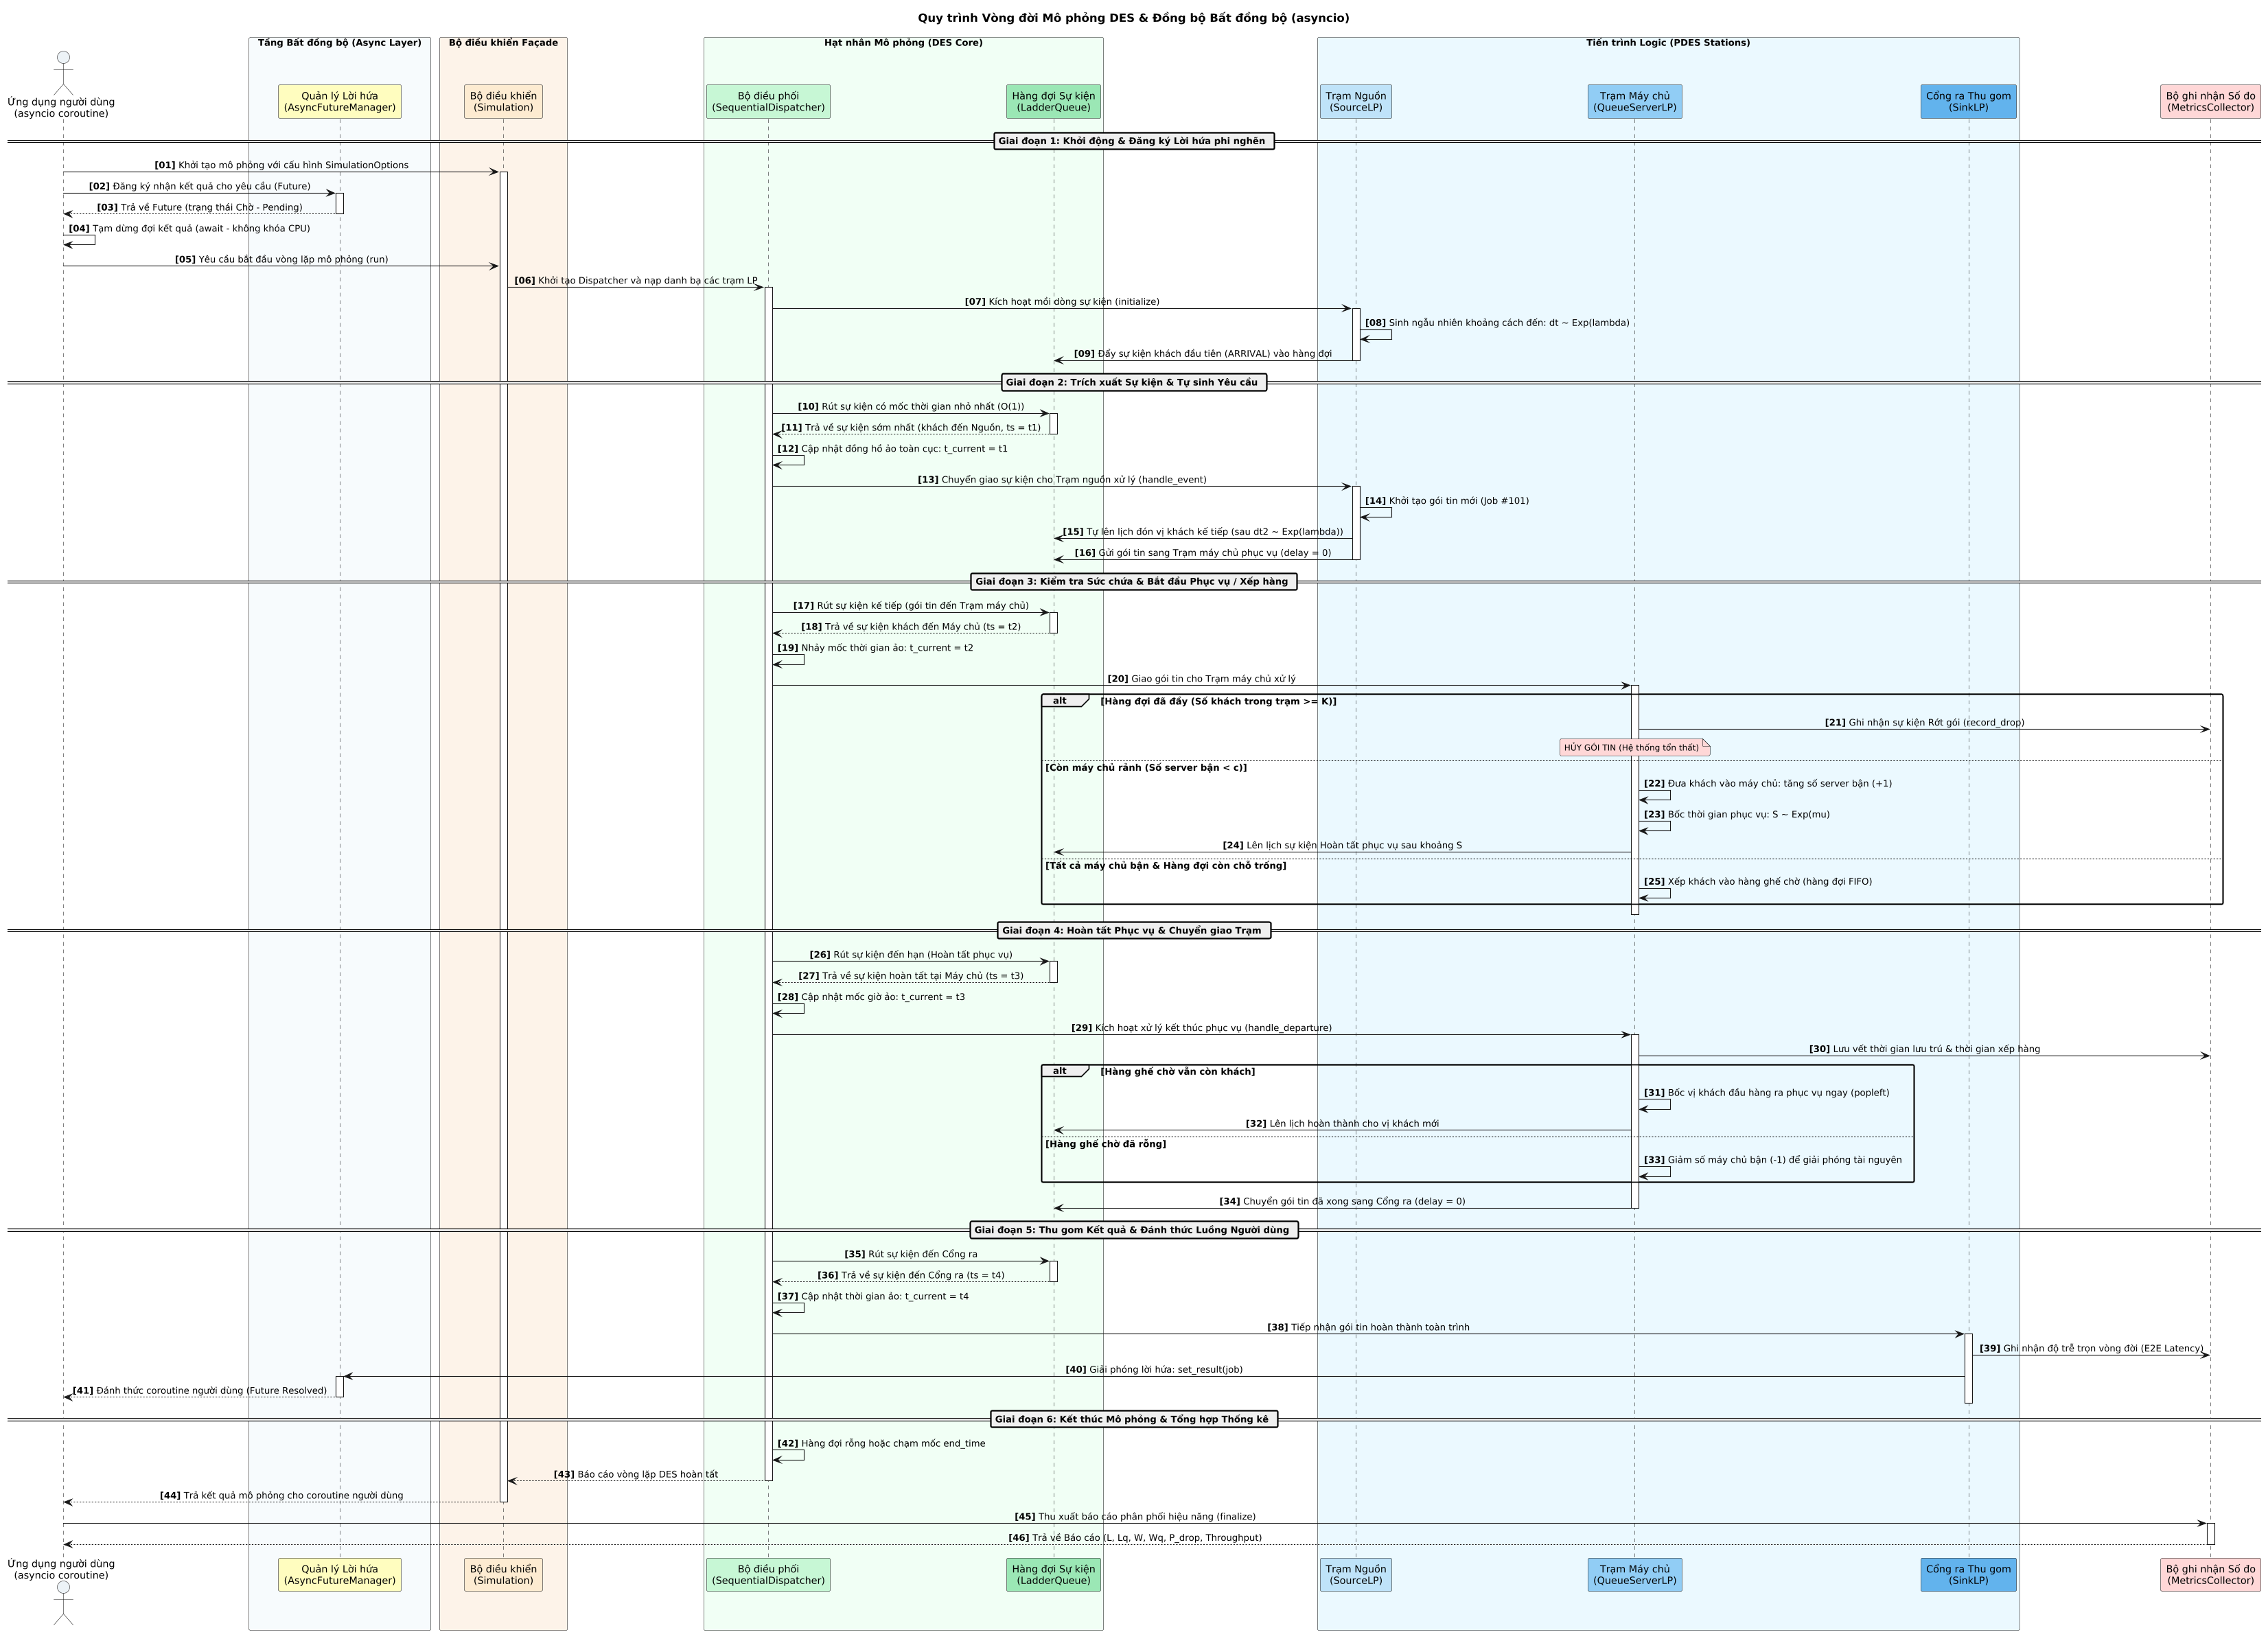
\includegraphics[width=0.95\textwidth]{image/uml_sequence_diagram.png}
\caption{Sơ đồ tuần tự luân chuyển sự kiện (UML Sequence Diagram) trong vòng lặp DES}
\label{fig:uml-sequence-diagram}
\end{figure}

Tiến trình điều phối và xử lý sự kiện trong sơ đồ tuần tự (Hình~\ref{fig:uml-sequence-diagram}) thiết lập cầu nối đồng bộ chặt chẽ giữa tầng ứng dụng bất đồng bộ và hạt nhân mô phỏng rời rạc. Nhằm làm rõ trách nhiệm kiến trúc và giải tỏa sự nhập nhằng giữa các không gian lưu trữ, vai trò cùng cấu trúc dữ liệu nội bộ của từng thực thể tham gia được chú thích chi tiết tại Bảng~\ref{tab:sequence-participants-annotated}.

\begin{table}[H]
\centering
\small
\renewcommand{\arraystretch}{1.25}
\setlength{\tabcolsep}{5pt}
\setlength{\aboverulesep}{0pt}
\setlength{\belowrulesep}{0pt}
\noindent\begin{tabularx}{\linewidth}{>{\small\bfseries\color{bkblue}\raggedright\arraybackslash}p{3.4cm} >{\small\ttfamily\raggedright\arraybackslash}p{3.8cm} >{\small\raggedright\arraybackslash}X}
\arrayrulecolor{bkblue}\toprule[1.5pt]
\rowcolor{bkblue}%
\multicolumn{1}{>{\raggedright\arraybackslash}p{3.4cm}}{\textbf{\color{white}Thành phần}} &
\multicolumn{1}{>{\raggedright\arraybackslash}p{3.8cm}}{\textbf{\color{white}Nơi lưu trữ nội bộ}} &
\multicolumn{1}{>{\raggedright\arraybackslash}X}{\textbf{\color{white}Vai trò \& Hành vi nghiệp vụ tương tác}} \\
\midrule[1pt]
\rowcolor{white}\texttt{User} (Script) & options: \newline SimulationOptions & Điểm khởi tạo cấu hình, nạp mô hình vào Facade và kích hoạt điều phối. \\
\rowcolor{boxbg}\texttt{App} (Coroutine) & -- & Tác vụ coroutine phía người dùng; phát yêu cầu và tạm dừng bằng \texttt{await future} phi phong tỏa luồng. \\
\rowcolor{white}\texttt{Simulation} (Sim) & options, models, \newline lps, dispatcher & Lớp mặt tiền (Facade) quản lý chu trình sống, nạp tự động các LP và kết nối Dispatcher. \\
\rowcolor{boxbg}\texttt{AsyncFutureManager} & \_pending\_futures: \newline Dict[int, Future] & Cầu nối bất đồng bộ; lưu trữ danh bạ lời hứa (\textit{Future}) để đánh thức coroutine khi có kết quả. \\
\rowcolor{white}\texttt{SequentialEvent-}\newline\texttt{Dispatcher} & current\_time, lps, \newline event\_queue, trace\_log & Bộ máy điều phối trung tâm; duy trì mốc $LVT$ toàn cục $t$, trích xuất sự kiện sớm nhất thúc đẩy bước nhảy thời gian. \\
\rowcolor{boxbg}\texttt{LadderQueue} & \_bottom, \_top, \newline \_boundary, bucket\_width & \textbf{Sổ lịch hẹn sự kiện}; hàng đợi ưu tiên phân tầng đạt chi phí $\mathcal{O}(1)$ lưu trữ các bản tin \texttt{Event}. \\
\rowcolor{white}\texttt{SourceLP} & local\_virt\_time, \newline \_started, \_job\_counter & Cổng phát sinh tải Poisson; khi mồi sự kiện sẽ tự động lên lịch đón vị khách kế tiếp sau $\Delta t \sim \text{Exp}(\lambda)$. \\
\rowcolor{boxbg}\texttt{QueueServerLP} & waiting\_queue (FIFO), \newline busy\_servers, metrics & Trạm máy chủ kèm bộ đệm; quản lý \textbf{hàng ghế chờ FIFO} lưu \texttt{Job} khi cả $c$ máy chủ đều bận. \\
\rowcolor{white}\texttt{SinkLP} & completed\_jobs, \newline total\_response\_times & Cổng ra thu gom; điểm kết thúc hành trình của \texttt{Job}, tính trễ toàn trình $W$ và kích hoạt giải phóng \texttt{Future}. \\
\rowcolor{boxbg}\texttt{MetricsCollector} & waiting\_times, \newline \_area\_q\_len, \_area\_in\_sys & Bộ tích lũy số đo; tính tích phân thời gian $\sum \text{State} \cdot \Delta t$ để xác định $W, W_q, L, L_q, \rho, P_b$. \\
\arrayrulecolor{bkblue}\bottomrule[1.5pt]
\end{tabularx}
\caption{Bảng chú thích vai trò và cấu trúc lưu trữ của các thực thể tham gia sơ đồ tuần tự}
\label{tab:sequence-participants-annotated}
\end{table}

Dựa trên sự phân công trách nhiệm rành mạch trên, toàn bộ tiến trình điều phối và luân chuyển sự kiện được phân tầng thành 6 giai đoạn kỹ thuật rõ rệt, gắn kết trực tiếp với các bước tương tác từ \textbf{[01]} đến \textbf{[46]}:

\begin{enumerate}[leftmargin=2em, itemsep=6pt]
\item \textbf{Giai đoạn 1: Khởi động \& Đăng ký Lời hứa phi nghẽn (Bước [01] -- [09]):}
\begin{itemize}[leftmargin=1.5em, itemsep=2pt]
\item \textit{Đăng ký Promise:} Coroutine phía người dùng gọi phương thức \texttt{register\_promise()} tới \texttt{AsyncFutureManager}. Trình quản lý khởi tạo đối tượng \texttt{asyncio.Future}, lưu trữ vào bảng tra cứu \texttt{\_pending\_futures} và trao lại đối tượng này cho người dùng. Ứng dụng thực hiện \texttt{await future} để tạm dừng luồng gọi mà hoàn toàn không phong tỏa luồng điều phối chính.
\item \textit{Mồi luồng sự kiện:} Hệ thống kích hoạt phương thức \texttt{start()} tại trạm \texttt{SourceLP}. Trạm nguồn bốc mẫu ngẫu nhiên khoảng thời gian đến đầu tiên $\Delta t_1 \sim \text{Exp}(\lambda)$, đóng gói thành bản tin \texttt{Event(type=ARRIVAL, dest='Source', timestamp=$\Delta t_1$)} và đẩy trực tiếp vào hàng đợi ưu tiên \texttt{EventQueue}.
\end{itemize}

\item \textbf{Giai đoạn 2: Trích xuất Sự kiện \& Tự sinh Yêu cầu (Bước [10] -- [16]):}
\begin{itemize}[leftmargin=1.5em, itemsep=2pt]
\item \textit{Bước nhảy thời gian ảo:} \texttt{Dispatcher} thực hiện thao tác \texttt{queue.pop()} lấy sự kiện có nhãn thời gian sớm nhất ra khỏi \texttt{EventQueue} và cập nhật trục thời gian ảo toàn cục: $t_{\text{current}} = t_1$. Mọi khoảng thời gian trống từ $0.00$ đến $t_1$ được bỏ qua tức thời.
\item \textit{Tự sinh dòng Poisson vô hạn:} Sự kiện được chuyển giao cho \texttt{SourceLP} để khởi tạo một thực thể \texttt{Job} mới (chứa mã định danh \texttt{job\_id} và mốc giờ đến \texttt{arrival\_time} = $t_1$). Đồng thời, trạm tự lên lịch cho chính mình sự kiện khách đến kế tiếp sau độ trễ $\Delta t_2 \sim \text{Exp}(\lambda)$ và ném vào \texttt{EventQueue} nhằm duy trì dòng khách liên tục. Ngay sau đó, trạm chuyển tiếp gói tin sang \texttt{QueueServerLP} với độ trễ chuyển mạch bằng 0 (tức thời tại mốc $t_1$).
\end{itemize}

\item \textbf{Giai đoạn 3: Phân phối \& Kiểm tra Sức chứa tại Máy chủ (Bước [17] -- [25]):}
\begin{itemize}[leftmargin=1.5em, itemsep=2pt]
\item \texttt{Dispatcher} tiếp tục lấy sự kiện đến chuyển cho \texttt{QueueServerLP.handle\_event(e)}.
\item \textit{Cơ chế kiểm soát đệm $K$:} Máy chủ kiểm tra ngưỡng dung lượng trạm: nếu số khách hiện hữu trong trạm (bao gồm số khách đang được phục vụ cộng với số khách đang ngồi chờ) đã đạt trần $K$ ($N(t) = \text{busy} + \text{len(waiting\_queue)} \ge K$), gói tin bị hủy bỏ ngay lập tức (\textit{Packet Dropped}) và cập nhật tổn thất vào \texttt{MetricsCollector}.
\item \textit{Phân bổ phục vụ hoặc xếp hàng chờ:} Nếu trạm còn chỗ:
\begin{itemize}[leftmargin=1.2em, itemsep=1pt]
\item Khi có ít nhất một máy chủ rảnh rỗi ($\text{busy\_servers} < c$): Yêu cầu \texttt{Job} được đưa thẳng vào phục vụ ngay (thời gian chờ $W_q = 0$). Trạm tăng bộ đếm $\text{busy\_servers} \leftarrow \text{busy\_servers} + 1$, bốc ngẫu nhiên thời gian phục vụ $S \sim \text{Exp}(\mu)$ và tạo sự kiện hoàn tất trong tương lai \texttt{Event(type=DEPARTURE, timestamp=$t + S$)} đẩy vào \texttt{EventQueue}.
\item Khi tất cả $c$ máy chủ đều đang bận ($\text{busy\_servers} = c$): Yêu cầu \texttt{Job} được đưa vào \textbf{hàng ghế chờ FIFO} \texttt{waiting\_queue.append(job)} nằm bên trong trạm để kiên nhẫn đợi đến lượt.
\end{itemize}
\end{itemize}

\item \textbf{Giai đoạn 4: Hoàn tất Phục vụ \& Chuyển giao Trạm (Bước [26] -- [34]):}
\begin{itemize}[leftmargin=1.5em, itemsep=2pt]
\item Khi trục thời gian ảo tiến tới mốc hoàn thành $t_{\text{current}} = t + S$, \texttt{Dispatcher} kích hoạt sự kiện \texttt{DEPARTURE} tại \texttt{QueueServerLP}.
\item Máy chủ ghi nhận thời gian lưu trú và thời gian chờ vào \texttt{MetricsCollector}. Sau đó kiểm tra hàng ghế chờ:
\begin{itemize}[leftmargin=1.2em, itemsep=1pt]
\item Nếu \texttt{waiting\_queue} còn khách: Trạm lập tức bốc vị khách đầu hàng ra xử lý (\texttt{waiting\_queue.popleft()}), bốc thời gian phục vụ mới $S'$ và lên lịch sự kiện \texttt{DEPARTURE} tiếp theo vào \texttt{EventQueue}.
\item Nếu \texttt{waiting\_queue} rỗng: Trạm giảm bộ đếm máy chủ bận ($\text{busy\_servers} \leftarrow \max(0, \text{busy} - 1)$) để hoàn trả tài nguyên máy chủ về trạng thái rảnh rỗi.
\end{itemize}
\item Gói tin đã xử lý xong được chuyển tiếp sang cổng ra \texttt{SinkLP} với độ trễ bằng 0.
\end{itemize}

\item \textbf{Giai đoạn 5: Thu gom Kết quả \& Giải phóng Lời hứa (Bước [35] -- [41]):}
\begin{itemize}[leftmargin=1.5em, itemsep=2pt]
\item \texttt{SinkLP} tiếp nhận gói tin hoàn tất, tính toán độ trễ toàn trình $T = t_{\text{dep}} - t_{\text{arr}}$ và ghi nhận vào \texttt{MetricsCollector}.
\item Trạm gọi phương thức \texttt{set\_result(job\_id, job)} trên \texttt{AsyncFutureManager}. Trình quản lý tra cứu mã yêu cầu trong bảng \texttt{\_pending\_futures}, gán giá trị kết quả và giải phóng \texttt{Future}. Lập tức coroutine phía người dùng đang dừng ở lệnh \texttt{await} được đánh thức để nhận kết quả trong thời gian thực mà không làm phong tỏa tiến trình mô phỏng rời rạc.
\end{itemize}

\item \textbf{Giai đoạn 6: Kết thúc Mô phỏng \& Tổng hợp Thống kê (Bước [42] -- [46]):}
\begin{itemize}[leftmargin=1.5em, itemsep=2pt]
\item Khi chạm mốc thời gian kết thúc $T_{\text{end}}$ hoặc \texttt{EventQueue} cạn kiệt phần tử, \texttt{Dispatcher} dừng vòng lặp điều phối và phát thông báo hoàn tất tới ứng dụng.
\item Ứng dụng người dùng kích hoạt phương thức trích xuất báo cáo từ \texttt{MetricsCollector} để thu được toàn bộ vector chỉ số hiệu năng chuẩn xác ($W, W_q, L, L_q, P_b, \lambda_{\text{eff}}$).
\end{itemize}
\end{enumerate}

\begin{table}[H]
\centering
\small
\renewcommand{\arraystretch}{1.35}
\setlength{\tabcolsep}{5pt}
\setlength{\aboverulesep}{0pt}
\setlength{\belowrulesep}{0pt}
\noindent\begin{tabularx}{\linewidth}{>{\ttfamily\bfseries\color{bkblue}\raggedright\arraybackslash}p{2.2cm} >{\ttfamily\raggedright\arraybackslash}p{3.2cm} >{\ttfamily\raggedright\arraybackslash}p{2.6cm} >{\centering\arraybackslash}p{1.6cm} >{\raggedright\arraybackslash}X}
\arrayrulecolor{bkblue}\toprule[1.5pt]
\rowcolor{bkblue}%
\multicolumn{1}{>{\raggedright\arraybackslash}p{2.2cm}}{\textbf{\color{white}Kiểu sự kiện}} &
\multicolumn{1}{>{\raggedright\arraybackslash}p{3.2cm}}{\textbf{\color{white}Thực thể phát}} &
\multicolumn{1}{>{\raggedright\arraybackslash}p{2.6cm}}{\textbf{\color{white}Thực thể nhận}} &
\multicolumn{1}{>{\centering\arraybackslash}p{1.6cm}}{\textbf{\color{white}Độ trễ $\Delta t$}} &
\multicolumn{1}{>{\raggedright\arraybackslash}X}{\textbf{\color{white}Hành vi nghiệp vụ kích hoạt}} \\
\midrule[1pt]
\rowcolor{white}ARRIVAL & SourceLP & SourceLP & $\text{Exp}(\lambda)$ & Tự sinh khách kế tiếp và duy trì dòng Poisson \\
\rowcolor{boxbg}ARRIVAL & SourceLP & QueueServerLP & $0.0$ & Chuyển Job mới đến kiểm tra dung lượng bộ đệm $K$ \\
\rowcolor{white}DEPARTURE & QueueServerLP & QueueServerLP & $\text{Exp}(\mu)$ & Hoàn tất phục vụ, giải phóng server, đón khách chờ \\
\rowcolor{boxbg}ARRIVAL & BranchingServerLP & Printer / Disk & $0.0$ & Rẽ nhánh xác suất ($p=0.3$ Máy in, $p=0.7$ Ổ đĩa) \\
\rowcolor{white}ARRIVAL & Server / Disk & SinkLP & $0.0$ & Ghi nhận trễ toàn trình và kích hoạt \texttt{set\_result()} \\
\rowcolor{boxbg}TERMINATE & Dispatcher & Dispatcher & $T_{\text{end}}$ & Dừng vòng lặp điều phối và tổng kết kết quả \\
\arrayrulecolor{bkblue}\bottomrule[1.5pt]
\end{tabularx}
\caption{Ma trận thông điệp sự kiện luân chuyển giữa các thành phần}
\label{tab:sequence-matrix}
\end{table}

% Ma trận trên khẳng định hai đặc tính then chốt trong cơ chế luân chuyển sự kiện:
% \begin{itemize}[leftmargin=1.5em, itemsep=2pt]
% \item \textbf{Phân ly lỏng (Loose Coupling):} Các trạm logic hoàn toàn không gọi trực tiếp phương thức của nhau mà chỉ tương tác gián tiếp thông qua việc phát sinh bản tin \texttt{Event} đẩy vào hàng đợi trung tâm.
% \item \textbf{Đồng bộ bước nhảy thời gian:} Ngoại trừ các sự kiện có độ trễ ngẫu nhiên (sinh khách $\text{Exp}(\lambda)$ và phục vụ $\text{Exp}(\mu)$), mọi sự kiện chuyển tiếp nội bộ giữa các trạm đều được xử lý với độ trễ chuyển mạch bằng 0 (tức thời tại cùng mốc thời gian ảo).
% \end{itemize}


% \textbf{Kịch bản số học minh họa trực quan tiến trình luân chuyển sự kiện (Trace Walkthrough):}

% Để làm sáng tỏ tính tương tác giữa các thành phần trong không gian thời gian ảo, kịch bản dưới đây minh họa vết thực thi số học cụ thể trên cấu hình hàng đợi đơn máy chủ $M/M/1/5$ ($c=1, K=5$) qua Bảng~\ref{tab:numerical-trace-walkthrough}:

% \begin{table}[H]
% \centering
% \small
% \renewcommand{\arraystretch}{1.3}
% \setlength{\tabcolsep}{5pt}
% \setlength{\aboverulesep}{0pt}
% \setlength{\belowrulesep}{0pt}
% \noindent\begin{tabularx}{\linewidth}{>{\centering\arraybackslash\bfseries\color{bkblue}}p{1.7cm} >{\ttfamily\raggedright\arraybackslash}p{2.3cm} >{\ttfamily\raggedright\arraybackslash}p{2.5cm} >{\centering\arraybackslash}p{2.8cm} >{\raggedright\arraybackslash}X}
% \arrayrulecolor{bkblue}\toprule[1.5pt]
% \rowcolor{bkblue}%
% \multicolumn{1}{>{\centering\arraybackslash}p{1.8cm}}{\textbf{\color{white}Mốc giờ $t$}} &
% \multicolumn{1}{>{\raggedright\arraybackslash}p{2.3cm}}{\textbf{\color{white}Sự kiện kích hoạt}} &
% \multicolumn{1}{>{\raggedright\arraybackslash}p{2.5cm}}{\textbf{\color{white}Trạm xử lý}} &
% \multicolumn{1}{>{\centering\arraybackslash}p{2.8cm}}{\textbf{\color{white}Trạng thái trạm}} &
% \multicolumn{1}{>{\raggedright\arraybackslash}X}{\textbf{\color{white}Hành vi nghiệp vụ \& Biến động số đo}} \\
% \midrule[1pt]
% \rowcolor{white}$t = 0.00$ & Khởi động & SourceLP & $\text{busy}=0, Q=0$ & Mồi hệ thống: sinh $\Delta t_1 = 1.20$, đẩy $e_1(\text{ARRIVAL}, t=1.20)$ vào \texttt{EventQueue}. \\
% \rowcolor{boxbg}$t = 1.20$ & ARRIVAL (Source) & SourceLP & $\text{busy}=0, Q=0$ & Khởi tạo yêu cầu $J_1$, tự hẹn khách $J_2$ tại $t=2.80$, chuyển $J_1$ sang trạm máy chủ. \\
% \rowcolor{white}$t = 1.20$ & ARRIVAL (Server) & QueueServerLP & $\text{busy}=1, Q=0$ & Máy chủ rảnh $\to$ phục vụ $J_1$ ngay ($W_{q,1} = 0.00$). Bốc $S_1 = 1.50$, hẹn xong tại $t=2.70$. \\
% \rowcolor{boxbg}$t = 2.70$ & DEPARTURE & QueueServerLP & $\text{busy}=0, Q=0$ & Hoàn tất $J_1$, giải phóng máy chủ (hàng chờ rỗng), chuyển $J_1$ sang cổng ra \texttt{SinkLP}. \\
% \rowcolor{white}$t = 2.70$ & ARRIVAL (Sink) & SinkLP & $\text{busy}=0, Q=0$ & Ghi nhận độ trễ $T_1 = 1.50$s. Gọi \texttt{set\_result()} $\to$ Đánh thức coroutine \texttt{await}. \\
% \rowcolor{boxbg}$t = 2.80$ & ARRIVAL (Server) & QueueServerLP & $\text{busy}=1, Q=0$ & Khách $J_2$ đến; do máy chủ đã giải phóng tại $t=2.70$, $J_2$ được phục vụ ngay lập tức. \\
% \arrayrulecolor{bkblue}\bottomrule[1.5pt]
% \end{tabularx}
% \caption{Bảng diễn biến vết thực thi sự kiện số học (Numerical Trace Walkthrough)}
% \label{tab:numerical-trace-walkthrough}
% \end{table}

% Qua bảng diễn biến trên, hai đặc tính then chốt của kiến trúc DES được kiểm chứng rõ nét:
% \begin{itemize}[leftmargin=1.5em, itemsep=2pt]
% \item \textbf{Tính phi nghẽn tuyệt đối:} Mọi tính toán diễn ra tức thời tại các mốc biến cố rời rạc ($0.00 \to 1.20 \to 2.70 \to 2.80$). Trục thời gian máy tính không hề bị lãng phí cho các khoảng thời gian hệ thống nhàn rỗi ($t \in (0.00, 1.20)$ hay $t \in (2.70, 2.80)$).
% \item \textbf{Tính bảo toàn nhân quả:} Không xuất hiện bất kỳ sự kiện nào có mốc thời gian ngược về quá khứ; trật tự các bước tuân thủ nghiệm ngặt thứ tự ưu tiên của hàng đợi Min-Heap.
% \end{itemize}
\newpage
% =========================================================================
\subsection{Kiến trúc điều phối cốt lõi của bộ mô phỏng DES (Core DES Dispatching Architecture)}
\label{subsec:core-des-engine}
% =========================================================================
\subsubsection{Cấu trúc Lớp Bản ghi Sự kiện (\texttt{Event}) và Cơ chế So sánh theo Thời gian ảo (Timestamp Ordering)}
\label{subsubsec:event-structure}

\hspace{0.5cm}Trong mô phỏng DES, toàn bộ động thái của hệ thống được kích hoạt bằng các bản tin sự kiện (\texttt{Event}). Để tối ưu hóa hiệu năng trích xuất và bảo đảm tính tiền định (\textit{Determinism}), hệ thống áp dụng cơ chế so sánh tự nhiên dựa trên mốc thời gian ảo \texttt{timestamp}:

\begin{equation}
e_1 < e_2 \iff e_1.\text{timestamp} < e_2.\text{timestamp}
\end{equation}
trong đó:
\begin{itemize}[leftmargin=2em, itemsep=1pt]
\item $e.\text{timestamp}$: Mốc thời gian ảo mà sự kiện sẽ nổ ra (tiêu chí so sánh tự nhiên duy nhất theo khai báo \texttt{@dataclass(order=True)}).
\item $e.\text{sender\_id}$: Mã định danh tiến trình logic phát sinh sự kiện (hỗ trợ alias property \texttt{source\_lp}).
\item $e.\text{receiver\_id}$: Mã định danh tiến trình logic tiếp nhận sự kiện (hỗ trợ alias property \texttt{dest\_lp}).
\item $e.\text{event\_type}$: Kiểu sự kiện trong mô hình rời rạc (\texttt{ARRIVAL}, \texttt{SERVICE\_START}, \texttt{DEPARTURE},...).
\item $e.\text{payload}$: Tải trọng dữ liệu đi kèm gói tin (chứa đối tượng \texttt{Job} hoặc từ điển dữ liệu, hỗ trợ alias property \texttt{data}).
\item $e.\text{event\_id}$: Chuỗi định danh duy nhất của sự kiện dạng UUID4 tự sinh.
\end{itemize}

\begin{lstlisting}[language=Python, caption={Cấu trúc sự kiện Event và cơ chế so sánh theo thời gian ảo (bkitevsim/core/event.py)}, label={lst:event-core}]
from __future__ import annotations
from dataclasses import dataclass, field
from enum import Enum, auto
import uuid
from typing import Any, Optional

class EventType(Enum):
    """Event types supported in discrete-event queuing models."""
    ARRIVAL = auto()        # Customer or packet arrives at a station
    SERVICE_START = auto()  # Server starts servicing a waiting customer
    DEPARTURE = auto()      # Service complete; packet departs station
    IO_COMPLETE = auto()    # I/O peripheral data transfer completed
    MESSAGE = auto()        # Inter-LP asynchronous coordination message
    TERMINATE = auto()      # Triggers simulation engine termination

@dataclass(order=True)
class Event:
    """Represents a discrete event in the simulation (PDES model).

    Events are ordered by timestamp for priority queue operations.
    The order=True parameter generates natural comparison based on timestamp.
    """
    # --- 1st key: Earliest virtual time (LVT) ---
    timestamp: float
    # --- Domain attributes (excluded from heap comparisons via compare=False) 
    sender_id: Any = field(compare=False, default=0)
    receiver_id: Any = field(compare=False, default=0)
    event_type: Any = field(compare=False, default="EVENT")
    payload: Any = field(compare=False, default=None)
    event_id: Any = field(compare=False, default_factory=lambda: str(uuid.uuid4()))

    def __init__(
        self,
        timestamp: float = 0.0,
        sender_id: Any = None,
        receiver_id: Any = None,
        event_type: Any = "EVENT",
        payload: Any = None,
        event_id: Any = None,
        **kwargs: Any
    ) -> None:
        self.timestamp = float(timestamp)
        # Handle source / sender aliases
        self.sender_id = sender_id if sender_id is not None else kwargs.get("source_lp", 0)
        # Handle destination / receiver aliases
        self.receiver_id = receiver_id if receiver_id is not None else kwargs.get("dest_lp", 0)
        self.event_type = event_type.name if hasattr(event_type, "name") else str(event_type)
        self.payload = payload if payload is not None else kwargs.get("data", None)
        self.event_id = str(event_id) if event_id is not None else str(uuid.uuid4())
        self._priority = kwargs.get("priority", 0)

        # Validation: Enforce non-negative timestamps
        if self.timestamp < 0:
            raise ValueError(f"Event timestamp cannot be negative: {self.timestamp}")

    @property
    def source_lp(self) -> Any:
        return self.sender_id

    @property
    def dest_lp(self) -> Any:
        return self.receiver_id
\end{lstlisting}

\newpage
\textbf{Phân tích kỹ thuật chuyên sâu về Phòng vệ kiểu dữ liệu và Cơ chế so sánh trong \texttt{bkitevsim}:}

Để hiểu rõ tại sao kiến trúc lớp \texttt{Event} trong gói \texttt{bkitevsim} mang tính quyết định đến độ ổn định của toàn bộ hệ thống mô phỏng, cần phân tích nguy cơ kỹ thuật tiềm ẩn trong các hệ thống DES hướng đối tượng:
\begin{itemize}[leftmargin=1.5em, itemsep=3pt]
\item \textbf{Cơ chế định thời tự nhiên qua \texttt{@dataclass(order=True)}:} Tiêu chí cốt lõi của DES là nguyên lý nhân quả: sự kiện có mốc thời gian ảo nhỏ hơn bắt buộc phải được trích xuất và kích hoạt trước. Bằng cách khai báo \texttt{timestamp: float} là trường so sánh duy nhất và kích hoạt \texttt{order=True}, Python tự động sinh các phương thức so sánh quan hệ (\texttt{\_\_lt\_\_}, \texttt{\_\_gt\_\_},...) thuần túy dựa trên biến số thực \texttt{timestamp}, giúp các cấu trúc hàng đợi ưu tiên (\texttt{MinHeapPriorityQueue} và \texttt{LadderQueue}) đạt tốc độ so sánh cực đại $\mathcal{O}(1)$ trên thanh ghi CPU.
\item \textbf{Phòng vệ ngoại lệ thời gian chạy (\textit{Runtime Exception Prevention}):} Nhờ thiết lập \texttt{compare=False}, trong ngôn ngữ Python, nếu hai đối tượng dataclass có trường so sánh đầu tiên bằng nhau ($e_1.\text{timestamp} == e_2.\text{timestamp}$), module \texttt{heapq} sẽ tự động so sánh trường tiếp theo được định nghĩa trong lớp. Nếu không thiết lập tường minh, bộ so sánh sẽ chạm vào trường \texttt{payload} chứa kiểu dữ liệu từ điển (\texttt{dict}) hoặc đối tượng nghiệp vụ phức tạp. Do Python không hỗ trợ toán tử so sánh $<$ giữa hai từ điển, chương trình sẽ lập tức ném ngoại lệ:
\begin{center}
\texttt{TypeError: '<' not supported between instances of 'dict'}
\end{center}
làm sập toàn bộ tiến trình mô phỏng ngay tại thời gian chạy. Trong gói \texttt{bkitevsim}, việc cấu hình tường minh \texttt{compare=False} cho toàn bộ các trường còn lại (\texttt{sender\_id}, \texttt{receiver\_id}, \texttt{event\_type}, \texttt{payload}, \texttt{event\_id}) là giải pháp phòng vệ kiến trúc mang tính sống còn, cô lập hoàn toàn phép so sánh heap chỉ vào biến số thực \texttt{timestamp}.
\item \textbf{Hệ thống thuộc tính tương thích ngược (\textit{Backward Compatibility Properties}):} Nhằm dung hòa giữa chuẩn thiết kế mới của gói \texttt{bkitevsim} (sử dụng danh pháp chuẩn PDES \texttt{sender\_id}, \texttt{receiver\_id}, \texttt{payload}) và các kịch bản mô phỏng kiểm thử cũ, lớp \texttt{Event} cung cấp sẵn hệ thống getter property (\texttt{source\_lp}, \texttt{dest\_lp}, \texttt{data}, \texttt{priority}), cho phép mã nguồn ngoài truy cập nhất quán mà không làm thay đổi cấu trúc lưu trữ nội bộ.
\end{itemize}

\newpage
\subsubsection{Cấu trúc hàng đợi sự kiện phân tầng hai cấp (LadderQueue)}
\label{subsubsec:ladder-queue}

\hspace{0.5cm}Cấu trúc Min-Heap nhị phân chuẩn sở hữu chi phí chèn và xóa là $O(\log N)$. Khi số lượng sự kiện mô phỏng vượt ngưỡng $10^6$, độ sâu của cây Heap làm suy giảm nghiêm trọng băng thông xử lý của CPU.

Để giải quyết vấn đề này, nhóm đã hiện thực thuật toán \textbf{\texttt{LadderQueue}} phân tầng hai cấp (Hình~\ref{fig:ladder-queue-arch}):
\begin{itemize}[leftmargin=1.5em, itemsep=3pt]
\item \textbf{Tầng dưới (\texttt{\_bottom}):} Lưu trữ tập hợp các sự kiện sắp xảy ra trong một cửa sổ thời gian gần $[t_{\text{current}}, \text{\_boundary}]$. Do số lượng phần tử nhỏ, thao tác trích xuất đạt hiệu năng tối ưu $O(1)$.
\item \textbf{Tầng trên (\texttt{\_top}):} Lưu trữ các sự kiện thuộc tương lai xa ($t > \text{\_boundary}$).
\item \textbf{Bất biến phân tầng (\textit{Tiered Invariant}):} Duy trì đẳng thức:
\begin{equation}
\max_{e \in \text{\_bottom}} (e.\text{timestamp}) \le \text{\_boundary} < \min_{e \in \text{\_top}} (e.\text{timestamp})
\end{equation}
\item \textbf{Cơ chế nạp tầng (\textit{Rung Refill}):} Khi tầng \texttt{\_bottom} cạn kiệt, thuật toán xác định ranh giới mới $\text{\_boundary} = \min(\text{\_top}) + \text{rung\_width}$ và trút các sự kiện thỏa điều kiện từ tầng trên xuống tầng dưới.
\end{itemize}

\begin{figure}[H]
\centering
\begin{tikzpicture}[scale=0.92, every node/.style={transform shape}]
% ==============================================================
% 1. TẦNG TRÊN (TOP HEAP) - LƯU SỰ KIỆN TƯƠNG LAI
% ==============================================================
% Khung bao ngoai Top Heap (shifted by +0.9)
\draw[thick, fill=gray!6, draw=gray!60, rounded corners=6pt] (0, 6.2) rectangle (14.6, 8.7);

% Header banner Top Heap
\path[fill=gray!22, rounded corners=6pt] (0, 8.0) rectangle (14.6, 8.7);
\path[fill=gray!22] (0, 8.0) rectangle (14.6, 8.2);
\draw[draw=gray!50, thick] (0, 8.0) -- (14.6, 8.0);

\node[anchor=west, font=\bfseries\footnotesize\color{black!80}] at (0.35, 8.35) 
{TẦNG ĐỈNH: Top Heap ($t > \text{boundary}$)};
\node[anchor=east, font=\scriptsize\bfseries, fill=gray!75!black, text=white, rounded corners=3pt, inner sep=3.5pt] at (14.25, 8.35) 
{Min-Heap: $\mathcal{O}(\log N)$};

% Cac the su kien trong Top Heap
\draw[fill=white, draw=gray!70, rounded corners=3pt, line width=0.8pt] (0.6, 6.7) rectangle (2.2, 7.7);
\node[font=\footnotesize\bfseries\color{black!85}] at (1.4, 7.35) {$e_5$};
\node[font=\scriptsize\color{black!70}] at (1.4, 6.95) {$t = 5.6$};

\draw[fill=white, draw=gray!70, rounded corners=3pt, line width=0.8pt] (2.5, 6.7) rectangle (4.1, 7.7);
\node[font=\footnotesize\bfseries\color{black!85}] at (3.3, 7.35) {$e_6$};
\node[font=\scriptsize\color{black!70}] at (3.3, 6.95) {$t = 7.2$};

\draw[fill=white, draw=gray!70, rounded corners=3pt, line width=0.8pt] (4.4, 6.7) rectangle (6.0, 7.7);
\node[font=\footnotesize\bfseries\color{black!85}] at (5.2, 7.35) {$e_7$};
\node[font=\scriptsize\color{black!70}] at (5.2, 6.95) {$t = 8.9$};

\draw[fill=white, draw=gray!70, rounded corners=3pt, line width=0.8pt] (6.3, 6.7) rectangle (7.9, 7.7);
\node[font=\footnotesize\bfseries\color{black!85}] at (7.1, 7.35) {$e_8$};
\node[font=\scriptsize\color{black!70}] at (7.1, 6.95) {$t = 12.4$};

\node[font=\Large\bfseries\color{gray!80}] at (8.6, 7.2) {$\cdots$};

\draw[fill=white, draw=gray!70, rounded corners=3pt, line width=0.8pt] (9.3, 6.7) rectangle (11.1, 7.7);
\node[font=\footnotesize\bfseries\color{black!85}] at (10.2, 7.35) {$e_N$};
\node[font=\scriptsize\color{black!70}] at (10.2, 6.95) {$t = 4980.2$};

% The chu thich dac tinh Top Heap ben phai
\draw[fill=gray!15, draw=gray!40, rounded corners=3pt] (11.5, 6.7) rectangle (14.1, 7.7);
\node[font=\scriptsize\bfseries\color{black!75}] at (12.8, 7.35) {Cấu trúc Min-Heap};
\node[font=\tiny\color{black!60}] at (12.8, 6.95) {Độ sâu cây: $\sim \log_2 N$};

\node[anchor=west, font=\scriptsize\itshape\color{black!60}] at (0.6, 6.42) 
{* Lưu trữ $N$ sự kiện phát sinh xa trong tương lai; giảm thiểu tần suất tái sắp xếp cho CPU};

% ==============================================================
% 2. VÙNG CHUYỂN TIẾP: CƠ CHẾ NẠP TẦNG (RUNG REFILL)
% ==============================================================
% Hop thong tin Rung Refill o giua (shifted by +0.5)
\draw[fill=orange!7, draw=orange!75!black, line width=1pt, rounded corners=5pt] (1.5, 4.3) rectangle (13.1, 5.5);
\node[font=\bfseries\scriptsize\color{orange!95!black}] at (7.3, 5.15) 
{CƠ CHẾ NẠP TẦNG (RUNG REFILL) --- Kích hoạt khi Tầng Đáy rỗng};
\node[font=\scriptsize\color{black!85}] at (7.3, 4.80) 
{1. Thiết lập mốc mới: $\text{\_boundary} \leftarrow \min(e.\text{timestamp} \in \text{\_top}) + \text{rung\_width}$};
\node[font=\scriptsize\color{black!85}] at (7.3, 4.48) 
{2. Di chuyển các sự kiện thỏa $t \in [\min(\text{top}), \text{\_boundary}]$ nạp xuống Tầng Đáy};

% Mui ten nap tang ket noi Top Heap -> Rung Refill -> Bottom Rung (Length = 0.7 each!)
\draw[->, >=stealth, line width=1.8pt, color=orange!85!black] (4.0, 6.2) -- (4.0, 5.5);
\draw[->, >=stealth, line width=1.8pt, color=orange!85!black] (10.6, 6.2) -- (10.6, 5.5);
\draw[->, >=stealth, line width=1.8pt, color=orange!85!black] (4.0, 4.3) -- (4.0, 3.6);
\draw[->, >=stealth, line width=1.8pt, color=orange!85!black] (10.6, 4.3) -- (10.6, 3.6);

% ==============================================================
% 3. TẦNG DƯỚI (BOTTOM RUNG) - CỬA SỔ THỰC THI NHANH
% ==============================================================
% Khung bao ngoai Bottom Rung
\draw[thick, fill=blue!4, draw=bkblue!80, rounded corners=6pt] (0, 1.0) rectangle (14.6, 3.6);

% Header banner Bottom Rung
\path[fill=bkblue!15, rounded corners=6pt] (0, 2.9) rectangle (14.6, 3.6);
\path[fill=bkblue!15] (0, 2.9) rectangle (14.6, 3.1);
\draw[draw=bkblue!50, thick] (0, 2.9) -- (14.6, 2.9);

\node[anchor=west, font=\bfseries\footnotesize\color{bkblue}] at (0.35, 3.25) 
{TẦNG ĐÁY: Bottom Rung ($t \le \text{boundary}$)};
\node[anchor=east, font=\scriptsize\bfseries, fill=bkblue, text=white, rounded corners=3pt, inner sep=3.5pt] at (14.25, 3.25) 
{Thao tác Pop / Push: $\bm{\mathcal{O}(1)}$};

% The su kien trong Bottom Rung
\draw[fill=white, draw=bkblue, rounded corners=3pt, line width=1pt] (0.6, 1.45) rectangle (2.2, 2.45);
\node[font=\footnotesize\bfseries\color{bkblue}] at (1.4, 2.1) {$e_1$};
\node[font=\scriptsize\color{black!80}] at (1.4, 1.7) {$t = 1.2$};

\draw[fill=white, draw=bkblue, rounded corners=3pt, line width=1pt] (2.5, 1.45) rectangle (4.1, 2.45);
\node[font=\footnotesize\bfseries\color{bkblue}] at (3.3, 2.1) {$e_2$};
\node[font=\scriptsize\color{black!80}] at (3.3, 1.7) {$t = 1.8$};

\draw[fill=white, draw=bkblue, rounded corners=3pt, line width=1pt] (4.4, 1.45) rectangle (6.0, 2.45);
\node[font=\footnotesize\bfseries\color{bkblue}] at (5.2, 2.1) {$e_3$};
\node[font=\scriptsize\color{black!80}] at (5.2, 1.7) {$t = 2.4$};

\draw[fill=white, draw=bkblue, rounded corners=3pt, line width=1pt] (6.3, 1.45) rectangle (7.9, 2.45);
\node[font=\footnotesize\bfseries\color{bkblue}] at (7.1, 2.1) {$e_4$};
\node[font=\scriptsize\color{black!80}] at (7.1, 1.7) {$t = 3.1$};

% Vach ngan ranh gioi boundary
\draw[red!75!black, line width=1.5pt, dashed] (8.4, 1.15) -- (8.4, 2.75);

% Hop chu thich ranh gioi
\draw[fill=red!7, draw=red!70!black, rounded corners=3pt, line width=0.8pt] (8.8, 1.35) rectangle (14.2, 2.55);
\node[anchor=west, font=\scriptsize\bfseries\color{red!80!black}] at (9.0, 2.25) 
{Mốc ranh giới: $\text{\_boundary} = 3.5$};
\node[anchor=west, font=\tiny\color{black!80}] at (9.0, 1.90) 
{Độ rộng cửa sổ: $\Delta = \text{rung\_width} = 2.0$};
\node[anchor=west, font=\tiny\itshape\color{black!60}] at (9.0, 1.58) 
{Sự kiện $t > 3.5$ lưu trữ tại Top Heap};

% ==============================================================
% 4. THAO TÁC POP SỰ KIỆN RA HẠT NHÂN MÔ PHỎNG (DES ENGINE)
% ==============================================================
\draw[->, >=stealth, line width=1.8pt, color=green!60!black] (1.4, 1.0) -- (1.4, 0.2);
\node[anchor=west, font=\footnotesize\bfseries\color{green!55!black}] at (1.8, 0.6) 
{Pop sự kiện sớm nhất $e_1$ ($t=1.2$) đạt $\bm{\mathcal{O}(1)} \longrightarrow$ Chuyển tới DES Engine thực thi};
\end{tikzpicture}
\caption{Kiến trúc phân tầng hai cấp và cơ chế nạp tầng (Rung Refill) của thuật toán LadderQueue}
\label{fig:ladder-queue-arch}
\end{figure}

\begin{lstlisting}[language=Python, caption={Hiện thực cấu trúc phân tầng LadderQueue (bkitevsim/core/priority\_queue.py)}, label={lst:ladder-queue}]
class LadderQueue(BaseEventQueue):
    def __init__(self, bucket_width: float = 1.0, rung_width: Optional[float] = None) -> None:
        self.bucket_width = rung_width if rung_width is not None else bucket_width
        self.rung_width = self.bucket_width
        self._bottom: List[Event] = []
        self._top: List[Event] = []
        self._boundary: float = -1.0
        self._count: int = 0

    def push(self, event: Event) -> None:
        self._count += 1
        if not self._bottom:
            if not self._top:
                self._boundary = event.timestamp + self.bucket_width
                heapq.heappush(self._bottom, event)
                return
            else:
                if event.timestamp <= self._boundary:
                    heapq.heappush(self._bottom, event)
                else:
                    heapq.heappush(self._top, event)
        else:
            if event.timestamp <= self._boundary:
                heapq.heappush(self._bottom, event)
            else:
                heapq.heappush(self._top, event)

    def pop(self) -> Event:
        if self._count == 0:
            raise IndexError("pop from empty LadderQueue")

        if not self._bottom:
            self._refill_bottom()

        event = heapq.heappop(self._bottom)
        self._count -= 1
        return event

    def _refill_bottom(self) -> None:
        if not self._top:
            return

        min_future_time = self._top[0].timestamp
        self._boundary = min_future_time + self.bucket_width

        remaining_top: List[Event] = []
        for ev in self._top:
            if ev.timestamp <= self._boundary:
                self._bottom.append(ev)
            else:
                remaining_top.append(ev)

        heapq.heapify(self._bottom)
        self._top = remaining_top
        heapq.heapify(self._top)
\end{lstlisting}

Bảng~\ref{tab:queue-complexity} tổng hợp sự so sánh định lượng về độ phức tạp giữa hai cấu trúc hàng đợi sự kiện.

\begin{table}[H]
\centering
\small
\renewcommand{\arraystretch}{1.35}
\setlength{\tabcolsep}{5pt}
\setlength{\aboverulesep}{0pt}
\setlength{\belowrulesep}{0pt}
\noindent\begin{tabularx}{\linewidth}{>{\raggedright\arraybackslash\bfseries\color{bkblue}}p{3.8cm} >{\centering\arraybackslash}p{2.1cm} >{\centering\arraybackslash}p{2.1cm} >{\centering\arraybackslash}p{1.4cm} >{\raggedright\arraybackslash}X}
\arrayrulecolor{bkblue}\toprule[1.5pt]
\rowcolor{bkblue}%
\multicolumn{1}{>{\raggedright\arraybackslash}p{3.8cm}}{\textbf{\color{white}Cấu trúc hàng đợi}} &
\multicolumn{1}{>{\centering\arraybackslash}p{2.1cm}}{\textbf{\color{white}Thao tác Push}} &
\multicolumn{1}{>{\centering\arraybackslash}p{2.1cm}}{\textbf{\color{white}Thao tác Pop}} &
\multicolumn{1}{>{\centering\arraybackslash}p{1.4cm}}{\textbf{\color{white}Bộ nhớ}} &
\multicolumn{1}{>{\raggedright\arraybackslash}X}{\textbf{\color{white}Quy mô mô phỏng}} \\
\midrule[1pt]
\rowcolor{white}\texttt{MinHeapPriorityQueue} & $\mathcal{O}(\log N)$ & $\mathcal{O}(\log N)$ & $\mathcal{O}(N)$ & Kịch bản nhỏ đến trung bình ($N < 50.000$ sự kiện) \\
\rowcolor{boxbg}\texttt{LadderQueue} (Hình~\ref{fig:ladder-queue-arch}) & $\bm{\mathcal{O}(1)}$ khấu hao & $\bm{\mathcal{O}(1)}$ khấu hao & $\mathcal{O}(N)$ & Kịch bản tải cực hạn ($N > 10^6$ sự kiện) \\
\arrayrulecolor{bkblue}\bottomrule[1.5pt]
\end{tabularx}
\caption{So sánh độ phức tạp tính toán giữa Min-Heap và LadderQueue}
\label{tab:queue-complexity}
\end{table}

\textbf{Phân tích chi phí khấu hao và Độ nhạy tham số $\text{rung\_width}$ ($\Delta$):}

Hiệu năng vượt trội của thuật toán \texttt{LadderQueue} được chứng minh qua hai khía cạnh lý thuyết và thực nghiệm:

\begin{itemize}[leftmargin=1.5em, itemsep=3pt]
\item \textbf{Chứng minh chi phí khấu hao $\mathcal{O}(1)$ (\textit{Amortized Complexity}):}
Xét vòng đời của $N$ sự kiện mô phỏng:
\begin{itemize}[leftmargin=1.2em, itemsep=1pt]
\item Mỗi sự kiện khi sinh ra chỉ được đẩy vào \texttt{\_top} tối đa 1 lần (chi phí $\mathcal{O}(\log N)$) hoặc đẩy thẳng vào \texttt{\_bottom} (chi phí $\mathcal{O}(\log k)$ với $k \ll N$).
\item Trong toàn bộ quá trình mô phỏng, mỗi phần tử từ \texttt{\_top} chỉ được trút xuống \texttt{\_bottom} đúng 1 lần duy nhất thông qua cơ chế nạp tầng \texttt{\_refill\_bottom}.
\item Tại tầng đáy \texttt{\_bottom}, số lượng sự kiện luôn bị chặn trên bởi kích thước cửa sổ $\Delta = \text{rung\_width}$, do đó thao tác trích xuất \texttt{heappop} diễn ra trên tập phần tử rất nhỏ, tiệm cận $\mathcal{O}(1)$.
\item Tổng khối lượng tính toán phân bổ cho $N$ phần tử đạt $\mathcal{O}(N)$, dẫn đến chi phí trung bình trên mỗi thao tác là $\mathcal{O}(1)$ khấu hao.
\end{itemize}
\item \textbf{Phân tích độ nhạy của tham số độ rộng bước thang $\Delta$ (\texttt{rung\_width}):}
\begin{itemize}[leftmargin=1.2em, itemsep=1pt]
\item Nếu $\Delta \to \infty$: Cửa sổ thời gian quá rộng, toàn bộ sự kiện đều đổ dồn vào tầng đáy, khiến \texttt{\_bottom} bị quá tải và cấu trúc suy biến ngược trở lại thành một Min-Heap nhị phân thông thường ($\mathcal{O}(\log N)$).
\item Nếu $\Delta \to 0$: Cửa sổ thời gian quá hẹp, tầng đáy liên tục rỗng, hệ thống phải gọi hàm \texttt{\_refill\_bottom} với tần suất dày đặc, làm tiêu tốn tài nguyên CPU vào các chu kỳ dịch chuyển phần tử giữa hai tầng.
\item \textit{Quy tắc cấu hình tối ưu:} Giá trị $\Delta$ cần thỏa mãn $\Delta \approx \frac{k}{\lambda}$ (với $\lambda$ là tốc độ khách đến trung bình và $k \in [2, 5]$). Với tốc độ lưu lượng chuẩn $\lambda = 1.0$, nhóm thiết lập $\text{rung\_width} = 2.0$, bảo đảm mỗi lần nạp tầng chứa từ 2 đến 4 sự kiện, tối đa hóa thông lượng xử lý của CPU.
\end{itemize}
\end{itemize}

\newpage
\subsubsection{Vòng lặp điều phối sự kiện trung tâm (Dispatcher Event Loop)}
\label{subsubsec:dispatcher-engine}

\hspace{0.5cm}Lớp \texttt{Dispatcher} đóng vai trò là nhạc trưởng trung tâm, duy trì vòng lặp thực thi của hệ thống mô phỏng. Toàn bộ tiến trình điều phối được chuẩn hóa trong Thuật toán 1.

\begin{tcolorbox}[colback=white, colframe=bkblue, halign title=flush left, title={\raggedright \textbf{Thuật toán 1: Vòng lặp điều phối sự kiện rời rạc (\texttt{SequentialEventDispatcher.run})}}, fonttitle=\bfseries]
\textbf{Đầu vào:} Hàng đợi sự kiện $\mathcal{Q}$ (\texttt{LadderQueue}), bảng ánh xạ tiến trình logic $\mathcal{L}$ (\texttt{self.lps}), mốc kết thúc $T_{end}$.\\
\textbf{Đầu ra:} Thống kê thời gian mô phỏng ảo (\texttt{simulation\_time}) và thời gian thực máy tính (\texttt{wall\_time}).
\begin{enumerate}[leftmargin=2em, label=\arabic*:, itemsep=2pt, topsep=4pt]
\item \textbf{while} $\mathcal{Q} \neq \emptyset$ \textbf{do}
\item \quad $e \leftarrow \mathcal{Q}.\text{pop}()$ \hfill \textit{\color{gray}// Lấy sự kiện có timestamp sớm nhất từ tầng đáy $\mathcal{O}(1)$}
\item \quad \textbf{if} $e.\text{timestamp} > T_{end}$ \textbf{then}
\item \quad\quad $\mathcal{Q}.\text{push}(e)$; \textbf{break} \hfill \textit{\color{gray}// Vượt ngưỡng thời gian mô phỏng, bảo toàn biên và dừng}
\item \quad \textbf{end if}
\item \quad $t_{\text{current}} \leftarrow e.\text{timestamp}$ \hfill \textit{\color{red!70!black}\textbf{// Bước nhảy thời gian ảo: Không dùng sleep!}}
\item \quad Ghi vết sự kiện $e$ vào \texttt{trace\_log} \hfill \textit{\color{gray}// Kiểm chứng vết thực thi đơn điệu}
\item \quad $LP_{dest} \leftarrow \mathcal{L}[e.\text{receiver\_id}]$ \hfill \textit{\color{gray}// Tra cứu trạm đích (hoặc qua thuộc tính $e.\text{dest\_lp}$)}
\item \quad $LP_{dest}.\text{set\_local\_virt\_time}(e.\text{timestamp})$ \hfill \textit{\color{gray}// Cập nhật mốc LVT nhân quả cho trạm}
\item \quad $LP_{dest}.\text{handle\_event}(e)$ \hfill \textit{\color{gray}// Chuyển giao sự kiện cho trạm đích xử lý}
\item \quad \textbf{for each} $e_{out} \in LP_{dest}.\text{get\_output\_events}()$ \textbf{do} $\mathcal{Q}.\text{push}(e_{out})$ \hfill \textit{\color{gray}// Thu gom sự kiện xuất xưởng}
\item \quad $\text{events\_processed} \leftarrow \text{events\_processed} + 1$
\item \textbf{end while}
\item \textbf{return} Báo cáo thống kê hiệu năng mô phỏng \texttt{self.stats}.
\end{enumerate}
\end{tcolorbox}

\begin{lstlisting}[language=Python, caption={Vòng lặp điều phối chính trong bkitevsim/dispatchers/sequential\_eventdispatcher.py}, label={lst:dispatcher-run}, basicstyle=\ttfamily\scriptsize, aboveskip=2pt, belowskip=3pt]
    def run(self, end_time: Optional[float] = None) -> Dict[str, Any]:
        """Run the simulation until end_time or no more events."""
        if end_time is not None:
            self.end_time = float(end_time)
        wall_start = time.perf_counter()
        self.schedule_initial_events()

        while not self.event_queue.is_empty():
            event = self.event_queue.pop()

            # [Phase 1]: Boundary check - preserve boundary event when simulation horizon reached
            if event.timestamp > self.end_time:
                self.event_queue.push(event)
                break

            # [Phase 2]: Instantaneous Virtual Clock Jump and audit trace logging
            self.current_time = event.timestamp

            if len(self.trace_log) < self.max_trace_entries:
                self.trace_log.append({
                    "seq": self.events_processed + 1,
                    "event_id": event.event_id,
                    "timestamp": event.timestamp,
                    "type": str(event.event_type),
                    "src": event.sender_id,
                    "dst": event.receiver_id
                })

            # [Phase 3]: Message Routing via destination LP lookup and LVT advance
            receiver = self.lps.get(event.receiver_id)
            if receiver is not None:
                receiver.set_local_virt_time(event.timestamp)
                receiver.handle_event(event)
                for ev in receiver.get_output_events():
                    self.schedule_event(ev)

            self.events_processed += 1

        for lp in self.lps.values():
            lp.finalize()

        wall_duration = time.perf_counter() - wall_start
        self.stats = {
            "simulation_time": self.current_time,
            "events_processed": self.events_processed,
            "wall_time": wall_duration,
            "end_time": self.end_time,
            "dispatcher": "sequential",
        }
        return self.stats
\end{lstlisting}

\textbf{Phân tích 3 pha vận hành cốt lõi của vòng lặp Dispatcher:}

Vòng lặp thực thi của lớp \texttt{Dispatcher} được cấu trúc hóa thành 3 pha nghiệp vụ khép kín:

\begin{enumerate}[leftmargin=1.8em, itemsep=1.5pt, topsep=1.5pt]
\item \textbf{Pha 1: Trích xuất sự kiện và Bảo toàn ranh giới biên (\textit{Boundary Invariant Preservation}):}
\begin{itemize}[leftmargin=1.2em, itemsep=0.5pt]
\item \textit{Trích xuất đỉnh hàng đợi:} Lấy sự kiện sớm nhất (\texttt{self.event\_queue.pop()}) từ tầng đáy của \texttt{LadderQueue} với độ phức tạp khấu hao $\mathcal{O}(1)$.
\item \textit{Kiểm tra ngưỡng dừng:} So sánh mốc thời gian sự kiện với cận biên kết thúc ($e.\text{timestamp} > \text{self.end\_time}$).
\item \textit{Bảo toàn trạng thái biên:} Đẩy ngược sự kiện lại hàng đợi qua \texttt{event\_queue.push(event)} trước khi ngắt vòng lặp (\texttt{break}), cho phép chạy nối tiếp kịch bản (\textit{Simulation Resumption}) mà không mất mát dữ liệu biên.
\end{itemize}

\item \textbf{Pha 2: Nhảy thời gian ảo và Ghi nhận nhật ký vết (\textit{Audit Logging}):}
\begin{itemize}[leftmargin=1.2em, itemsep=0.5pt]
\item \textit{Bước nhảy thời gian ảo:} Cập nhật đồng hồ toàn cục $\texttt{self.current\_time} = e.\text{timestamp}$ tức thời trong $\mathcal{O}(1)$, hoàn toàn không tiêu tốn chu kỳ chờ CPU thực tế.
\item \textit{Ghi nhận nhật ký vết:} Lưu bản ghi cấu trúc \texttt{\{"seq", "event\_id", "timestamp", "type", "src", "dst"\}} vào \texttt{trace\_log} (với chặn trên \texttt{max\_trace\_entries = 1000} bảo đảm an toàn bộ nhớ).
\item \textit{Kiểm chứng nhân quả:} Cung cấp bằng chứng số học phục vụ xác minh tính đơn điệu ngặt của trục thời gian ảo trong các bài kiểm thử tự động.
\end{itemize}

\item \textbf{Pha 3: Điều phối thông điệp tức thời $\mathcal{O}(1)$ (\textit{Message Routing}):}
\begin{itemize}[leftmargin=1.2em, itemsep=0.5pt]
\item \textit{Tra cứu trạm đích:} Truy xuất thực thể trạm nhận qua bảng băm \texttt{self.lps} với khóa \texttt{event.receiver\_id} (hoặc alias \texttt{dest\_lp}) trong $\mathcal{O}(1)$.
\item \textit{Cập nhật LVT trạm nhận:} Gọi \texttt{receiver.set\_local\_virt\_time(event.timestamp)} để đồng bộ mốc thời gian ảo cục bộ và phòng vệ luật nhân quả trước khi xử lý.
\item \textit{Chuyển giao quyền xử lý:} Kích hoạt phương thức xử lý \texttt{receiver.}\allowbreak\texttt{handle\_event(event)} theo chuẩn PDES.
\item \textit{Thu gom sự kiện xuất xưởng:} Thu thập sự kiện mới phát sinh qua \texttt{receiver.}\allowbreak\texttt{get\_output\_events()} và nạp lại vào hàng đợi qua \texttt{self.schedule\_event(ev)}.
\item \textit{Cập nhật chỉ số:} Tăng bộ đếm sự kiện (\texttt{self.events\_processed += 1}) phục vụ đo đạc thông lượng và tốc độ xử lý.
\end{itemize}
\end{enumerate}

\subsubsection{Bộ điều khiển mô phỏng Facade (Simulation \& SimulationOptions)}
\label{subsubsec:simulation-controller}

\hspace{0.5cm}Nhằm tuân thủ trọn vẹn mô hình tương tác hệ thống được đặc tả trong Hình 4 và Hình 5 của đề bài \textit{The Queuing Systems-based Performance Evaluation Project (hk261\_BKsyspeEvsim.pdf)}, hệ thống không yêu cầu người dùng phải tự tay kết nối và khởi tạo chi tiết từng thành phần rời rạc. Thay vào đó, gói thư viện \texttt{bkitevsim} cung cấp một lớp mặt tiền điều phối cấp cao nhất mang tên \textbf{\texttt{Simulation}} kết hợp với đối tượng cấu hình \textbf{\texttt{SimulationOptions}} (Listing~\ref{lst:simulation-core-class}):

\begin{lstlisting}[language=Python, caption={Hiện thực lớp điều khiển Facade Simulation và cấu hình SimulationOptions (bkitevsim/core/simulation.py)}, label={lst:simulation-core-class}, basicstyle=\ttfamily\scriptsize, aboveskip=2pt, belowskip=3pt]
class SimulationOptions:
    # Encapsulates simulation configuration options for bkitevsim
    def __init__(
        self,
        end_time: float = 100.0,
        dispatcher: str = "sequential",
        bucket_width: float = 1.0,
        log_level: str = "INFO",
        log_file: Optional[str] = None,
        stats_file: Optional[str] = None,
        verbose: bool = False,
        model_params: Optional[Dict[str, Any]] = None
    ) -> None:
        self.end_time: float = end_time
        self.dispatcher: str = dispatcher
        self.bucket_width: float = bucket_width
        self.log_level: str = log_level
        self.log_file: Optional[str] = log_file
        self.stats_file: Optional[str] = stats_file
        self.verbose: bool = verbose
        self.model_params: Dict[str, Any] = model_params or {}

    def to_dict(self) -> Dict[str, Any]:
        return {
            "end_time": self.end_time, "dispatcher": self.dispatcher,
            "bucket_width": self.bucket_width, "log_level": self.log_level,
            "log_file": self.log_file, "stats_file": self.stats_file,
            "verbose": self.verbose, "model_params": self.model_params,
        }

    @classmethod
    def from_dict(cls, data: Dict[str, Any]) -> SimulationOptions:
        return cls(**data)


class Simulation:
    # High-level simulation controller (Facade Pattern according to Figure 4)
    def __init__(
        self,
        options: Optional[SimulationOptions] = None,
        models: Optional[Dict[str, Type[BkSysLogicalProcess]]] = None,
        factories: Optional[Dict[str, Callable[..., BkSysLogicalProcess]]] = None
    ) -> None:
        self.options: SimulationOptions = options if options is not None else SimulationOptions()
        self.models: Dict[str, Type[BkSysLogicalProcess]] = dict(models) if models else {}
        self.factories: Dict[str, Callable[..., BkSysLogicalProcess]] = dict(factories) if factories else {}
        self.lps: Dict[Any, BkSysLogicalProcess] = {}
        self.dispatcher: Optional[SequentialEventDispatcher] = None

    def register_model(self, name: str, model_cls: Type[BkSysLogicalProcess]) -> None:
        self.models[name] = model_cls

    def create_lp(self, lp_id: int | str, model_name: str, **params: Any) -> BkSysLogicalProcess:
        if model_name in self.factories:
            lp = self.factories[model_name](lp_id, **params)
        elif model_name in self.models:
            lp = self.models[model_name](lp_id, **params)
        else:
            raise ValueError(f"Model '{model_name}' is not registered.")

        self.lps[lp_id] = lp
        if self.dispatcher is not None:
            self.dispatcher.register_lp(lp)
        return lp

    def _create_dispatcher(self) -> SequentialEventDispatcher:
        disp_type = self.options.dispatcher.lower()
        if disp_type in ("distributed", "distributed_sequential"):
            return DistributedEventDispatcher(
                end_time=self.options.end_time, bucket_width=self.options.bucket_width
            )
        return SequentialEventDispatcher(
            end_time=self.options.end_time, bucket_width=self.options.bucket_width
        )

    def run(self) -> Dict[str, Any]:
        if self.dispatcher is None:
            self.dispatcher = self._create_dispatcher()
            for lp in self.lps.values():
                if lp.lp_id not in self.dispatcher.lps:
                    self.dispatcher.register_lp(lp)
        return self.dispatcher.run()

    def get_statistics(self) -> Dict[str, Any]:
        stats: Dict[str, Any] = dict(self.dispatcher.stats if self.dispatcher else {})
        per_lp: Dict[str, Any] = {}
        for lp_id, lp in self.lps.items():
            if hasattr(lp, "get_metrics") and callable(getattr(lp, "get_metrics")):
                per_lp[str(lp_id)] = lp.get_metrics()
            elif hasattr(lp, "metrics"):
                metrics_obj = getattr(lp, "metrics")
                if hasattr(metrics_obj, "finalize") and callable(getattr(metrics_obj, "finalize")):
                    per_lp[str(lp_id)] = metrics_obj.finalize(self.options.end_time)
        stats["per_lp_stats"] = per_lp
        return stats
\end{lstlisting}

\textbf{Phân tích kiến trúc và 4 ưu thế cốt lõi của Bộ điều khiển Facade \texttt{Simulation}:}

\begin{enumerate}[leftmargin=1.8em, itemsep=3pt]
\item \textbf{Đóng gói tham số vận hành chuẩn hóa (\texttt{SimulationOptions}):}
Mọi tham số thực nghiệm (thời gian mô phỏng \texttt{end\_time}, kiểu điều phối \texttt{dispatcher}, cấu hình bậc thang LadderQueue \texttt{bucket\_width}, mức nhật ký \texttt{log\_level}) được tập trung hóa vào một dataclass có kiểu dữ liệu tường minh. Hai phương thức \texttt{to\_dict()} và \texttt{from\_dict()} cho phép hệ thống nạp kịch bản thực nghiệm trực tiếp từ tệp JSON hoặc dòng lệnh CLI một cách tự động, bảo đảm tính tái lập (\textit{Reproducibility}) tuyệt đối.

\item \textbf{Cơ chế đăng ký mô hình khai báo (\textit{Declarative Model Registration}):}
Thông qua \texttt{register\_model()} và \texttt{register\_factory()}, người dùng có thể định nghĩa các lớp trạm logic tùy biến hoặc hàm sinh thực thể (Factory). Phương thức \texttt{create\_lp(lp\_id, model\_name, **params)} áp dụng mẫu thiết kế \textit{Factory Pattern}, cho phép khởi tạo hàng loạt trạm logic với các tham số khác nhau (như tốc độ đến $\lambda$, tốc độ phục vụ $\mu$, số server $c$, sức chứa $K$) mà không cần quản lý thủ công các con trỏ bộ nhớ.

\item \textbf{Tự động hóa gắn kết bộ điều phối (\texttt{\_create\_dispatcher}):}
Dựa trên giá trị \texttt{options.dispatcher}, lớp \texttt{Simulation} tự động lựa chọn và khởi tạo đúng loại Dispatcher:
\begin{itemize}[leftmargin=1.2em, itemsep=1pt]
\item Nếu \texttt{options.dispatcher == "sequential"}: Cấp phát \texttt{SequentialEventDispatcher} với một hàng đợi \texttt{LadderQueue} tập trung toàn cục.
\item Nếu \texttt{options.dispatcher == "distributed\_sequential"}:\\ Cấp phát \texttt{DistributedEventDispatcher} với cấu trúc phân vùng hàng đợi cục bộ cho từng LP (\texttt{\_lp\_queues[lp\_id] = LadderQueue()}).
\end{itemize}
Toàn bộ danh bạ các trạm logic trong \texttt{self.lps} được tự động đăng ký vào Dispatcher qua phương thức \texttt{dispatcher.register\_lp(lp)}.

\item \textbf{Tích hợp hợp nhất số liệu hiệu năng (\texttt{get\_statistics}):}
Sau khi vòng lặp DES kết thúc, phương thức \texttt{get\_statistics()} thực hiện duyệt qua tất cả các tiến trình logic đã đăng ký, tự động gọi \texttt{get\_metrics()} hoặc \texttt{metrics.finalize(sim\_time)} để kết xuất bảng số đo hiệu năng toàn diện ($W, W_q, L, L_q, \rho, P_b$) dưới dạng từ điển hợp nhất \texttt{per\_lp\_stats}, phục vụ trực tiếp cho việc đối chiếu giải tích và xuất biểu đồ khoa học.
\end{enumerate}


% =========================================================================
\subsection{Hiện thực mô hình Tiến trình logic và Các trạm hàng đợi (PDES)}
\label{subsec:pdes-and-queuing-models}
% =========================================================================

\subsubsection{Lớp cơ sở Tiến trình logic và Cơ chế giao tiếp hướng thông điệp}
\label{subsubsec:logical-process-base}

\hspace{0.5cm}Theo mô hình mô phỏng phân tán PDES của Fujimoto, hệ thống không duy trì một trạng thái khổng lồ tập trung mà phân rã thành các \textbf{Tiến trình logic (\textit{Logical Processes -- LPs})} độc lập thông qua lớp cơ sở \texttt{BkSysLogicalProcess} (alias \texttt{LogicalProcess}). Mỗi LP đóng vai trò là một thực thể tự trị có các thuộc tính kỹ thuật sau:
\begin{itemize}[leftmargin=1.5em, itemsep=2pt]
\item \textbf{Khép kín trạng thái (\texttt{BkSysLogicalProcessState}):} Đóng gói toàn bộ dữ liệu trạng thái nội bộ, hỗ trợ chụp ảnh nhanh (\texttt{checkpoint()}), khôi phục trạng thái (\texttt{restore()}) và lưu vết từng bước chuyển dịch (\texttt{record\_step()}).
\item \textbf{Đồng hồ ảo nội bộ (\texttt{LVT}):} Mỗi trạm tự quản lý mốc thời gian ảo cục bộ \texttt{local\_virt\_time} (truy xuất qua property \texttt{local\_virtual\_time}). Phương thức \texttt{set\_local\_virt\_time(t)} bắt buộc kiểm tra điều kiện $t \ge \text{local\_virt\_time}$, bảo đảm không có hiện tượng thời gian thụt lùi ngược về quá khứ (\textit{Local Causality Constraint - LCC}).
\item \textbf{Cơ chế giao tiếp không phong tỏa (\texttt{send\_event}):} Các trạm không gọi hàm chéo trực tiếp của nhau mà đóng gói thông điệp thành đối tượng \texttt{Event} và chuyển cho bộ điều phối xử lý qua \texttt{self.dispatcher.schedule\_event(event)} hoặc lưu tạm vào danh sách đệm xuất xưởng \texttt{\_output\_events}.
\end{itemize}

\begin{lstlisting}[language=Python, caption={Lớp cơ sở LogicalProcess và kiểm soát LVT (bkitevsim/core/logical\_process.py)}, label={lst:logical-process-base}]
class BkSysLogicalProcessState:
    """Encapsulates the mutable state of a Logical Process.

    Supports checkpointing, cloning, and state restoration for PDES.
    """
    def __init__(self, **kwargs: Any) -> None:
        self._data: Dict[str, Any] = dict(kwargs)
        self.history: List[Dict[str, Any]] = []

    def get(self, key: str, default: Any = None) -> Any:
        return self._data.get(key, default)

    def set(self, key: str, value: Any) -> None:
        self._data[key] = value

    def checkpoint(self) -> Dict[str, Any]:
        """Create a deep-copy checkpoint of the state."""
        return copy.deepcopy(self._data)

    def restore(self, checkpoint: Dict[str, Any]) -> None:
        """Restore state from a previous checkpoint."""
        self._data = copy.deepcopy(checkpoint)


class BkSysLogicalProcess(abc.ABC):
    """Abstract base class for a BkSys Logical Process in PDES.

    Each LP has a unique ID and maintains its own Local Virtual Time (LVT).
    """
    def __init__(
        self,
        lp_id: int | str,
        initial_state: Optional[BkSysLogicalProcessState] = None
    ) -> None:
        self.lp_id = lp_id
        self.local_virt_time: float = 0.0
        self.state = initial_state if initial_state is not None else BkSysLogicalProcessState()
        self._output_events: List[Event] = []
        self._dispatcher: Optional[Any] = None

    def set_local_virt_time(self, local_virt_time: float) -> None:
        """Enforces Local Causality Constraint (LCC): time cannot travel backward."""
        if local_virt_time < self.local_virt_time:
            raise ValueError(
                f"Causality violation in LP {self.lp_id}: cannot travel backward "
                f"from {self.local_virt_time:.4f} to {local_virt_time:.4f}"
            )
        self.local_virt_time = local_virt_time

    def send_event(self, event: Event) -> None:
        """Send an event to another LP or buffer it for dispatcher."""
        if self._dispatcher is not None and hasattr(self._dispatcher, "schedule_event"):
            self._dispatcher.schedule_event(event)
        else:
            self._output_events.append(event)
\end{lstlisting}

\subsubsection{Kiến trúc trạm phục vụ hợp nhất 6 mô hình hàng đợi Kendall}
\label{subsubsec:unified-queue-server}

\hspace{0.5cm}Thay vì hiện thực rời rạc từng lớp phần mềm riêng lẻ cho mỗi bài toán, lớp \textbf{\texttt{QueueServerLP}} được xây dựng theo kiến trúc hợp nhất dựa trên ký hiệu chuẩn Kendall $A/S/c/K$. Bằng cách tham số hóa hai biến quyết định:
\begin{itemize}[leftmargin=1.5em, itemsep=2pt]
\item \texttt{num\_servers} ($c$): Số lượng máy chủ song song ($1 \le c \le \infty$).
\item \texttt{capacity} ($K$): Tổng sức chứa tối đa của hệ thống (phục vụ + ghế chờ).
\end{itemize}

Hệ thống hợp nhất toàn bộ 6 mô hình hàng đợi lý thuyết một cách nhất quán:
\begin{enumerate}[leftmargin=2em, itemsep=2pt]
\item \textbf{Mô hình $M/M/1$:} \texttt{num\_servers = 1, capacity = None} (1 server, hàng đợi vô hạn).
\item \textbf{Mô hình $M/M/1/K$:} \texttt{num\_servers = 1, capacity = K} (1 server, bộ đệm giới hạn $K$).
\item \textbf{Mô hình $M/M/\infty$:} \texttt{num\_servers = float('inf'), capacity = None} (Vô hạn máy chủ).
\item \textbf{Mô hình $M/M/n/n$:} \texttt{num\_servers = n, capacity = n} (Mô hình Erlang loss, $0$ ghế chờ).
\item \textbf{Mô hình $M/M/c$:} \texttt{num\_servers = c, capacity = None} ($c$ máy chủ, hàng đợi vô hạn).
\item \textbf{Mô hình $M/M/c/K$:} \texttt{num\_servers = c, capacity = K} ($c$ máy chủ, bộ đệm giới hạn $K$).
\end{enumerate}


\begin{lstlisting}[language=Python, caption={Hai nhánh xử lý nghiệp vụ cốt lõi trong QueueServerLP}, label={lst:queue-server-core}, basicstyle=\ttfamily\scriptsize, aboveskip=2pt, belowskip=3pt]
    def _handle_arrival(self, event: Event) -> None:
        """Process ARRIVAL event: checks buffer capacity, allocates server or enqueues."""
        job: Job = event.payload["job"] if isinstance(event.payload, dict) and "job" in event.payload else event.payload
        job.arrival_time = event.timestamp
        self.metrics.record_arrival()

        # Branch 1: Finite buffer capacity check (M/M/1/K, M/M/c/K, M/M/n/n)
        if self.capacity is not None and self.total_in_system >= self.capacity:
            self.metrics.record_drop()  # Drop packet when buffer is full
            self._notify_state(event.timestamp)
            return

        # Branch 2: Server dispatching and waiting queue logic
        if self.busy_servers < self.num_servers:
            self.busy_servers += 1
            self._start_service(job, event.timestamp)
        else:
            self.waiting_queue.append(job)  # Enqueue into FIFO waiting buffer

        self._notify_state(event.timestamp)

    def _handle_departure(self, event: Event) -> None:
        """Process DEPARTURE event: records metrics, routes job downstream, and serves next."""
        payload = event.payload if isinstance(event.payload, dict) else {}
        job: Job = payload.get("job")
        service_duration = payload.get("duration", 0.0)

        if job and job.start_service_time is not None:
            # Compute waiting time in queue: Wq = start_service - arrival_time
            wait_time = job.start_service_time - job.arrival_time
            self.metrics.record_completion(wait_time, service_duration)
            job.departure_time = event.timestamp

            out_ev = create_event(
                timestamp=event.timestamp,
                sender_id=self.lp_id,
                receiver_id=self.dest_lp_id,
                event_type="ARRIVAL",
                payload={"job": job, "wait_time": wait_time, "service_time": service_duration}
            )
            self.send_event(out_ev)

        # Serve next waiting customer from queue or mark server idle
        if self.waiting_queue:
            next_job = self.waiting_queue.popleft()
            self._start_service(next_job, event.timestamp)
        else:
            self.busy_servers = max(0, self.busy_servers - 1)

        self._notify_state(event.timestamp)
\end{lstlisting}

\textbf{Bảng đối chiếu tham số hóa hợp nhất cho 6 mô hình hàng đợi Kendall:}

Bảng~\ref{tab:kendall-unified-mapping} tổng hợp sự ánh xạ giữa 6 mô hình lý thuyết Kendall và các tham số cấu hình cụ thể trong lớp \texttt{QueueServerLP}.

\begin{table}[H]
\centering
\small
\renewcommand{\arraystretch}{1.35}
\setlength{\tabcolsep}{5pt}
\setlength{\aboverulesep}{0pt}
\setlength{\belowrulesep}{0pt}
\noindent\begin{tabularx}{\linewidth}{>{\centering\arraybackslash\bfseries\color{bkblue}}p{1.9cm} >{\centering\arraybackslash}p{2.2cm} >{\centering\arraybackslash}p{2.0cm} >{\centering\arraybackslash}p{2.3cm} >{\raggedright\arraybackslash}X}
\arrayrulecolor{bkblue}\toprule[1.5pt]
\rowcolor{bkblue}%
\multicolumn{1}{>{\centering\arraybackslash}p{1.9cm}}{\textbf{\color{white}Mô hình}} &
\multicolumn{1}{>{\centering\arraybackslash}p{2.2cm}}{\textbf{\color{white}\texttt{num\_servers} ($c$)}} &
\multicolumn{1}{>{\centering\arraybackslash}p{2.0cm}}{\textbf{\color{white}\texttt{capacity} ($K$)}} &
\multicolumn{1}{>{\centering\arraybackslash}p{2.3cm}}{\textbf{\color{white}Ghế chờ}} &
\multicolumn{1}{>{\raggedright\arraybackslash}X}{\textbf{\color{white}Cơ chế tổn thất / rớt gói}} \\
\midrule[1pt]
\rowcolor{white}$M/M/1$ & $1$ & \texttt{None} & Vô hạn ($\infty$) & Không có rớt gói ($P_b = 0$, bộ đệm vô hạn) \\
\rowcolor{boxbg}$M/M/1/K$ & $1$ & $K$ & $K - 1$ chỗ & Hủy gói khi tổng số khách trong trạm $\ge K$ \\
\rowcolor{white}$M/M/\infty$ & $\infty$ (\texttt{inf}) & \texttt{None} & Không cần ghế ($W_q = 0$) & Không rớt gói; mỗi khách có máy chủ phục vụ riêng \\
\rowcolor{boxbg}$M/M/n/n$ & $n$ & $n$ & Không có ghế ($0$ chỗ) & Rớt gói Erlang-B khi toàn bộ $n$ máy chủ đều bận \\
\rowcolor{white}$M/M/c$ & $c$ & \texttt{None} & Vô hạn ($\infty$) & Không rớt gói; xếp hàng Erlang-C khi bận cả $c$ máy chủ \\
\rowcolor{boxbg}$M/M/c/K$ & $c$ & $K$ & $K - c$ chỗ & Hủy gói khi tổng số khách đang phục vụ $+$ chờ $\ge K$ \\
\arrayrulecolor{bkblue}\bottomrule[1.5pt]
\end{tabularx}
\caption{Ánh xạ tham số cấu hình hợp nhất cho 6 mô hình hàng đợi Kendall}
\label{tab:kendall-unified-mapping}
\end{table}


\textbf{Máy trạng thái hữu hạn xử lý sự kiện trong QueueServerLP:}

Hai phương thức \texttt{\_handle\_arrival} và \texttt{\_handle\_departure} trong Listing~\ref{lst:queue-server-core} hiện thực hóa hai máy trạng thái khép kín được đặc tả qua sơ đồ chuyển trạng thái FSM (Hình~\ref{fig:fsm-queue-server}):

\begin{figure}[H]
\centering
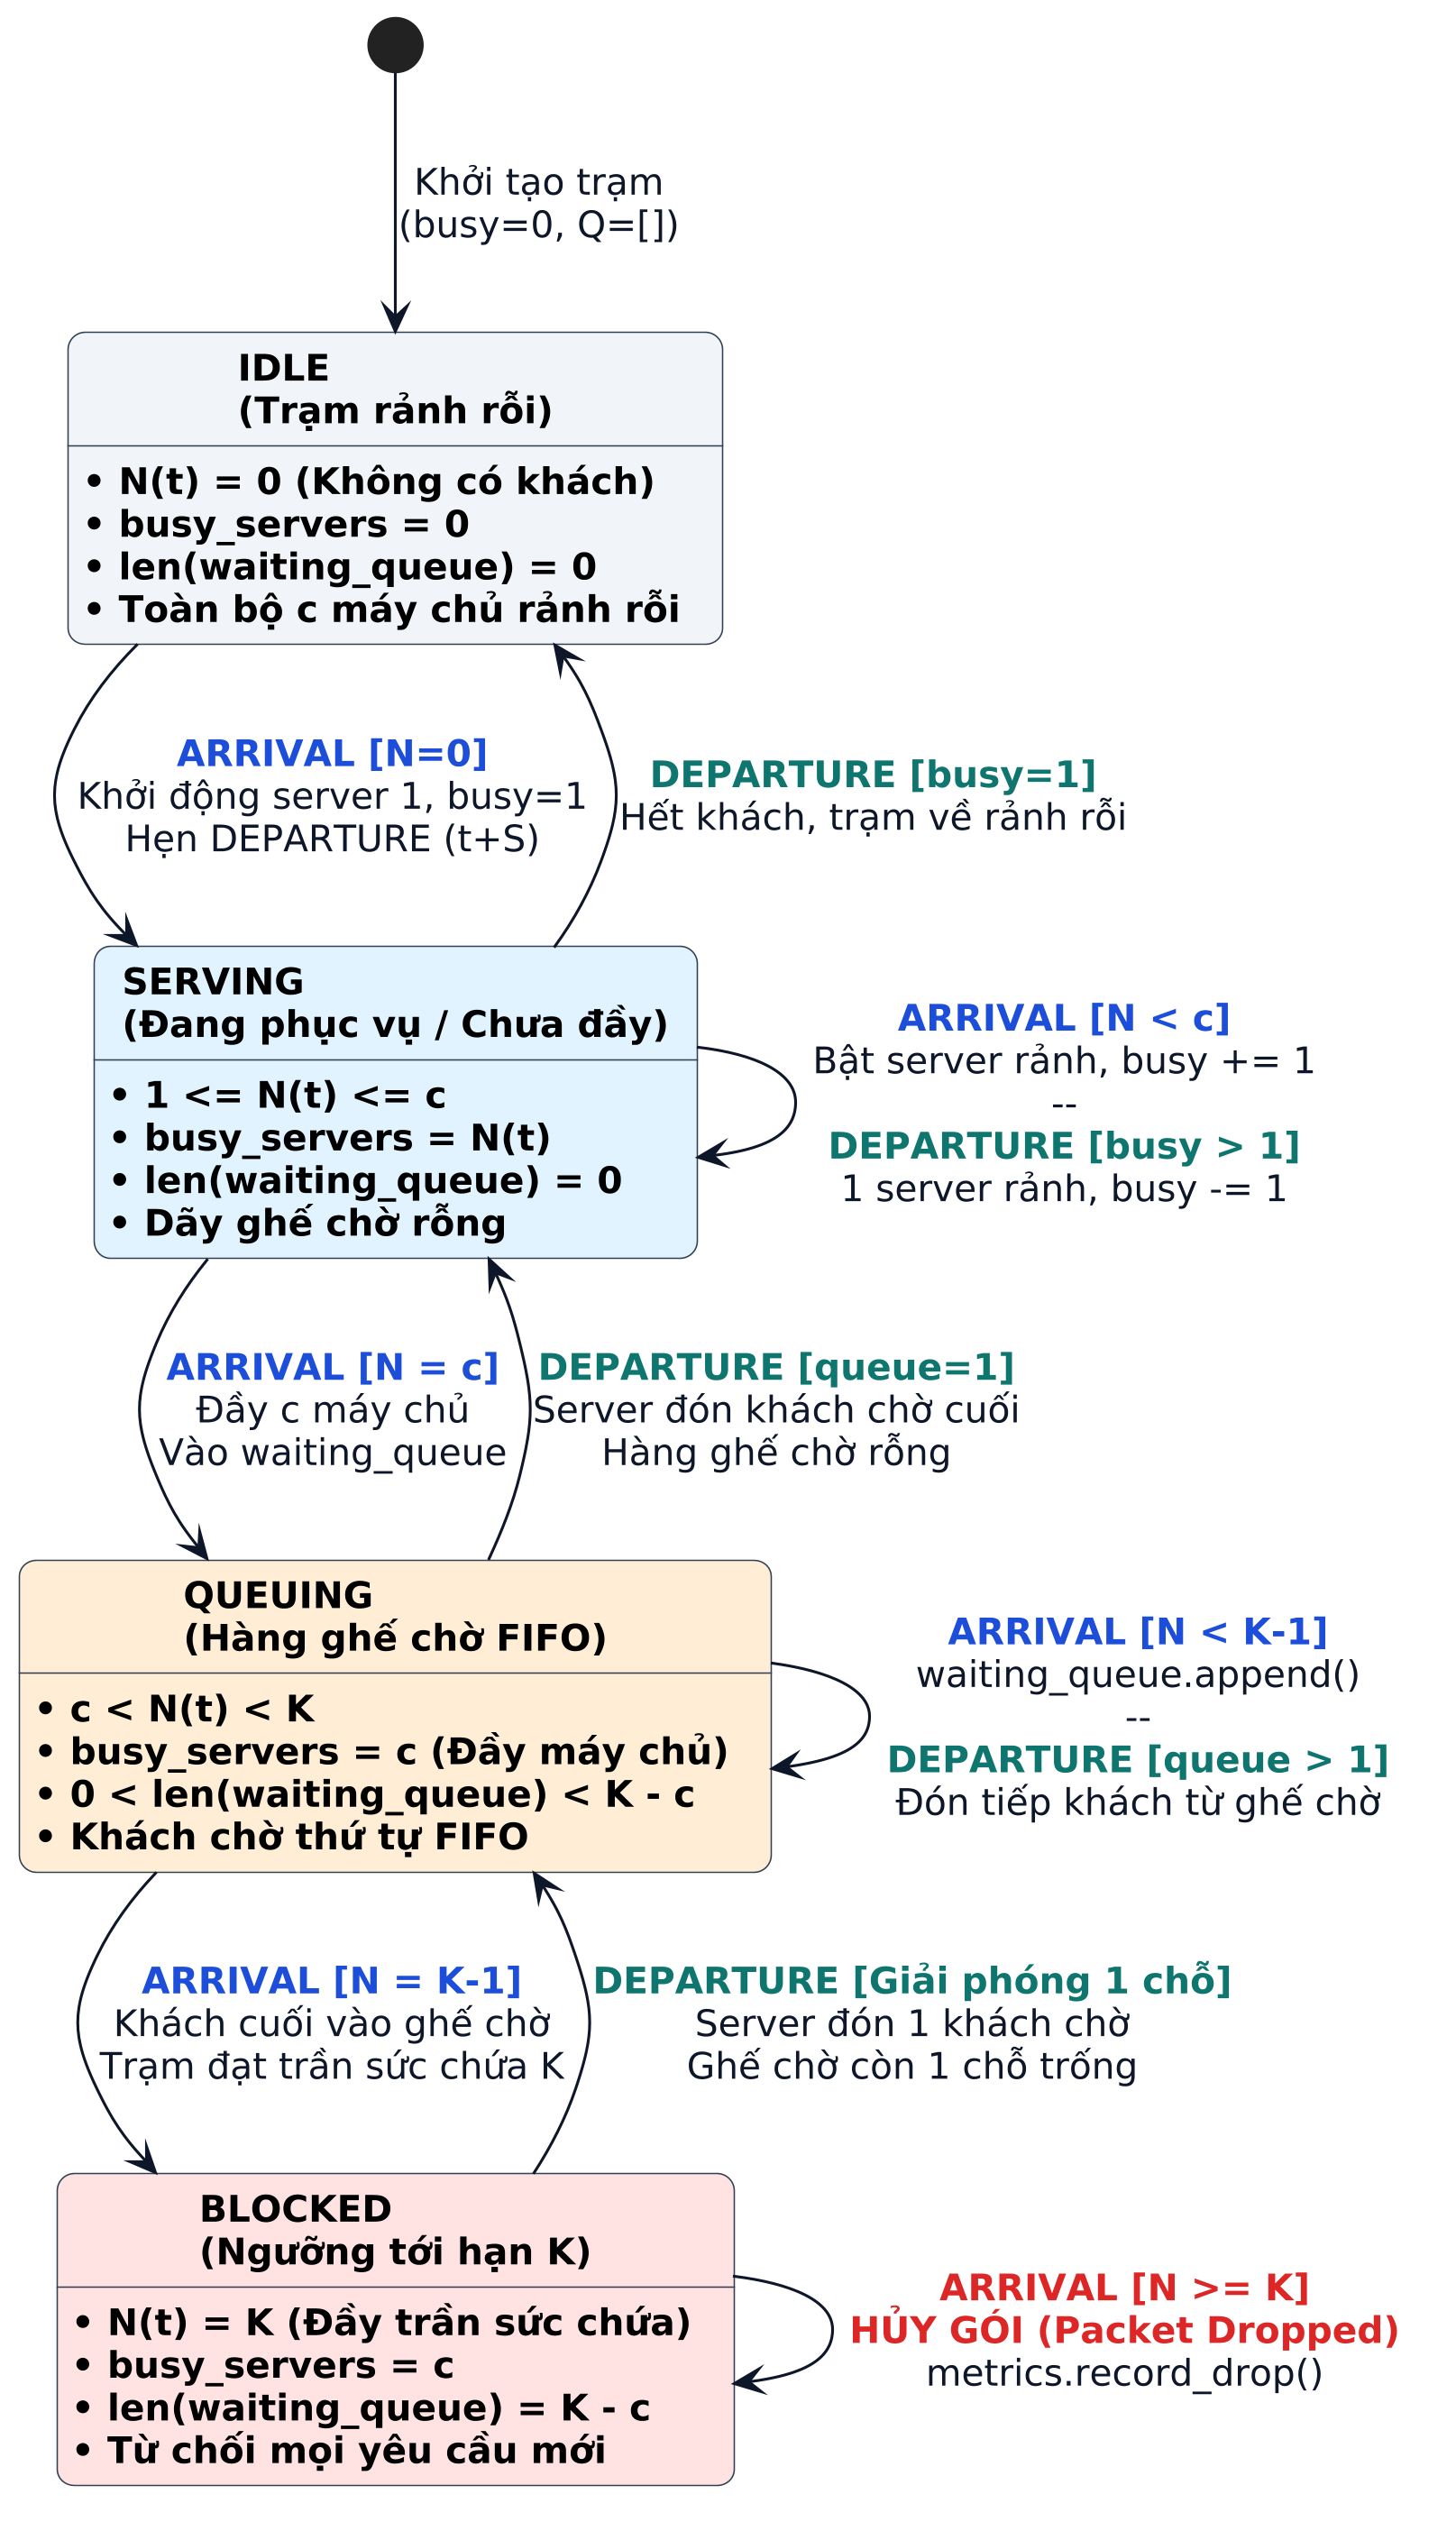
\includegraphics[width=0.6\textwidth]{image/fsm_queue_server_uml.png}
\caption{Máy trạng thái hữu hạn (FSM) mô hình hóa vòng đời phục vụ của \texttt{QueueServerLP}}
\label{fig:fsm-queue-server}
\end{figure}
\begin{itemize}[leftmargin=1.5em, itemsep=3pt]
\item \textbf{Máy trạng thái tiếp nhận (\texttt{\_handle\_arrival}):}
\begin{enumerate}[leftmargin=1.2em, label=\alph*)]
\item \textit{Kiểm tra sức chứa:} Tính tổng số khách trong trạm thông qua thuộc tính \texttt{total\_in\_system}, xác định bởi $N(t) = \text{busy} + |\mathcal{Q}_{\text{wait}}|$. Nếu $N(t) \ge K$ (với cấu hình có bộ đệm hữu hạn), trạm lập tức kích hoạt \texttt{self.metrics.record\_drop()} và hủy gói tin.
\item \textit{Điều phối máy chủ rảnh:} Nếu $\text{busy\_servers} < c$, trạm tăng số máy chủ bận thêm $1$ (\texttt{self.busy\_servers += 1}), bốc thời gian phục vụ $S \sim \text{Exp}(\mu)$ và phát sự kiện \texttt{DEPARTURE} trong tương lai qua \texttt{create\_event} với độ trễ $S$.
\item \textit{Xếp hàng chờ FIFO:} Nếu cả $c$ máy chủ đều bận, yêu cầu được đẩy vào hàng ghế chờ \texttt{waiting\_queue} bằng thao tác \texttt{append} đạt $\mathcal{O}(1)$.
\end{enumerate}
\item \textbf{Máy trạng thái hoàn tất (\texttt{\_handle\_departure}):}
\begin{enumerate}[leftmargin=1.2em, label=\alph*)]
\item \textit{Ghi nhận số liệu thống kê:} Tính thời gian chờ thực tế $W_q = t_{\text{start\_service}} - t_{\text{arrival}}$ và ghi nhận vào bộ tích lũy \texttt{MetricsCollector} qua phương thức \texttt{record\_completion(wait\_time, service\_duration)}.
\item \textit{Chuyển tiếp tác vụ:} Đóng gói đối tượng \texttt{Job} đã hoàn tất và phát sự kiện \texttt{ARRIVAL} tới trạm kế tiếp (\texttt{dest\_lp\_id}) qua \texttt{create\_event} với độ trễ $\Delta t = 0.0$.
\item \textit{Đón khách tiếp theo:} Nếu hàng chờ \texttt{waiting\_queue} còn khách, lấy phần tử đầu hàng qua \texttt{popleft()} ($\mathcal{O}(1)$) và phục vụ ngay. Nếu hàng rỗng, giảm biến đếm máy chủ bận: $\text{busy\_servers} \leftarrow \max(0, \text{busy\_servers} - 1)$.
\end{enumerate}
\end{itemize}

\subsubsection{Hiện thực mạng hàng đợi Jackson và Cơ chế rẽ nhánh xác suất}
\label{subsubsec:jackson-network-impl}

\hspace{0.5cm}Nhằm mô hình hóa mạng máy tính 4 nút trạm phức tạp theo Hình 1 của đề bài ($\text{Source} \to \text{I/O} \to \text{CPU} \to \text{Printer} / \text{Disk} \to \text{Sink}$), lớp \textbf{\texttt{BranchingServerLP}} kế thừa từ \texttt{QueueServerLP} và ghi đè logic hoàn tất phục vụ:

\begin{lstlisting}[language=Python, caption={Hiện thực rẽ nhánh xác suất trong BranchingServerLP (bkitevsim/models/network.py)}, label={lst:branching-server}]
class BranchingServerLP(QueueServerLP):
    """Probabilistic routing server modeling CPU departure branch in Jackson network."""

    def __init__(
        self,
        lp_id: int | str = "CPU",
        printer_lp_id: int | str = "Printer",
        disk_lp_id: int | str = "Disk",
        p_printer: float = 0.3,
        service_rate: float = 5.0,
        num_servers: float = 1,
        capacity: Optional[int] = None,
        metrics: Optional[MetricsCollector] = None
    ) -> None:
        super().__init__(
            lp_id=lp_id,
            dest_lp_id=printer_lp_id,
            service_rate=service_rate,
            num_servers=num_servers,
            capacity=capacity,
            metrics=metrics
        )
        self.printer_lp_id = printer_lp_id
        self.disk_lp_id = disk_lp_id
        self.p_printer = p_printer  # Probability of routing to Printer (0.3)

    def _handle_departure(self, event: Event) -> None:
        """Route departing job probabilistically via Bernoulli trial to Printer or Disk."""
        payload = event.payload if isinstance(event.payload, dict) else {}
        job: Job = payload.get("job")
        service_duration: float = payload.get("duration", 0.0)

        if job and job.start_service_time is not None:
            wait_time = job.start_service_time - job.arrival_time
            self.metrics.record_completion(wait_time, service_duration)
            job.departure_time = event.timestamp

            # Probabilistic routing: Bernoulli trial with probability p_printer
            dest = self.printer_lp_id if (random.random() < self.p_printer) else self.disk_lp_id
            if not hasattr(job, "orig_arrival_time"):
                job.orig_arrival_time = job.arrival_time
            job.arrival_time = event.timestamp

            out_ev = create_event(
                timestamp=event.timestamp,
                sender_id=self.lp_id,
                receiver_id=dest,
                event_type="ARRIVAL",
                payload={"job": job}
            )
            self.send_event(out_ev)

        if self.waiting_queue:
            next_job = self.waiting_queue.popleft()
            self._start_service(next_job, event.timestamp)
        else:
            self.busy_servers = max(0, self.busy_servers - 1)

        self._notify_state(event.timestamp)
\end{lstlisting}

\begin{itemize}[leftmargin=1.5em, itemsep=2pt]
\item \textbf{Cơ chế rẽ nhánh Bernoulli (\texttt{p\_printer}):} Tại ngã ba xuất phát từ CPU, bộ điều phối trạm thực hiện phép thử ngẫu nhiên: nếu $\text{random}() < p_{\text{printer}}$ (mặc định $0.3$) thì chuyển gói tin sang trạm \texttt{PrinterLP}, ngược lại ($1 - p = 0.7$) chuyển sang trạm \texttt{DiskLP}.
\item \textbf{Cơ chế bảo toàn mốc thời gian gốc (\texttt{orig\_arrival\_time}):} Khi gói tin chuyển tiếp qua các trạm I/O $\to$ CPU $\to$ Printer/Disk, thuộc tính \texttt{arrival\_time} được cập nhật tại chỗ để tính cục bộ $W_{q,\text{node}}$, trong khi \texttt{orig\_arrival\_time} được giữ nguyên vẹn giúp trạm đích \texttt{NetworkSinkLP} tính toán chính xác độ trễ toàn trình (\textit{End-to-End Latency}):
\begin{equation}
T_{\text{End-to-End}} = t_{\text{Sink}} - \text{job.orig\_arrival\_time}
\end{equation}
giúp đối chiếu trực tiếp với định lý Jackson giải tích: $W_{\text{network}} = W_{\text{IO}} + W_{\text{CPU}} + 0.3 W_{\text{Printer}} + 0.7 W_{\text{Disk}}$.
\end{itemize}

% =========================================================================
\subsection{Cơ chế giao tiếp phi nghẽn và Điều phối bất đồng bộ (Python Asyncio)}
\label{subsec:asyncio-implementation}
% =========================================================================

\subsubsection{Cơ chế giao tiếp phi nghẽn luồng theo mô hình Promise / Future}
\label{subsubsec:promise-future}

\hspace{0.5cm}Để kết nối giữa luồng gọi người dùng và bộ máy mô phỏng mà không gây nghẽn luồng chính (\textit{Non-blocking I/O}), lớp \textbf{\texttt{AsyncFutureManager}} hiện thực mẫu thiết kế Promise/Future:
\begin{itemize}[leftmargin=1.5em, itemsep=2pt]
\item \textbf{Khởi tạo và Quản lý Event Loop an toàn (\texttt{\_get\_loop}):} Tự động phát hiện vòng lặp sự kiện \texttt{asyncio} đang chạy hoặc tạo mới an toàn trên các phiên bản Python 3.10+, 3.11+ và 3.12+, tránh hoàn toàn lỗi \texttt{RuntimeError: no running event loop}.
\item \textbf{Tạo lời hứa (\texttt{create\_future}):} Khởi tạo một đối tượng \texttt{asyncio.Future} được gán nhãn duy nhất theo \texttt{request\_id} và lưu vào bảng tra cứu \texttt{\_pending\_futures}. Luồng gọi coroutine phía người dùng có thể thực hiện toán tử \texttt{await future} để tạm dừng tác vụ một cách hòa nhã mà không chiếm dụng CPU.
\item \textbf{Giải phóng lời hứa (\texttt{set\_result}):} Khi trạm thu gom \texttt{SinkLP} tiếp nhận kết quả cuối cùng của yêu cầu, phương thức \texttt{set\_result(request\_id, result)} lập tức hoàn tất Future và đánh thức coroutine đang chờ để nhận kết quả ngay tức thời.
\item \textbf{Báo lỗi và Hủy an toàn (\texttt{set\_exception}, \texttt{cancel\_all}):} Cho phép truyền trực tiếp đối tượng ngoại lệ vào Future khi gặp sự cố, hoặc hủy bỏ hàng loạt các lời hứa đang treo khi dừng hệ thống.
\end{itemize}

\begin{lstlisting}[language=Python, caption={Cơ chế Promise / Future phi nghẽn (bkitevsim/async\_engine/future\_manager.py)}, label={lst:future-manager}]
class AsyncFutureManager:
    """Manages asynchronous Request-to-Future lifecycle without thread blocking."""

    def __init__(self, loop: Optional[asyncio.AbstractEventLoop] = None) -> None:
        self.loop = loop
        # Pending future registry: mapping request_id -> asyncio.Future
        self._pending_futures: Dict[int, asyncio.Future] = {}

    def _get_loop(self) -> asyncio.AbstractEventLoop:
        """Retrieve active running event loop or create a fresh loop safely."""
        if self.loop is not None and not self.loop.is_closed():
            return self.loop
        try:
            return asyncio.get_running_loop()
        except RuntimeError:
            loop = asyncio.new_event_loop()
            asyncio.set_event_loop(loop)
            self.loop = loop
            return loop

    def create_future(self, request_id: int) -> asyncio.Future:
        """Create and register an asyncio.Future attached to a unique request ID."""
        loop = self._get_loop()
        future = loop.create_future()
        self._pending_futures[request_id] = future
        return future

    def set_result(self, request_id: int, result: Any) -> bool:
        """Resolve promise with result, awakening awaiting coroutine."""
        future = self._pending_futures.pop(request_id, None)
        if future and not future.done():
            future.set_result(result)
            return True
        return False
\end{lstlisting}

\subsubsection{Các mẫu điều phối đồng quy có cấu trúc (Structured Concurrency)}
\label{subsubsec:structured-concurrency}

\hspace{0.5cm}Từ phiên bản Python 3.11+, cơ chế \textbf{Structured Concurrency} qua \texttt{asyncio.TaskGroup} được áp dụng để quản lý an toàn vòng đời coroutine. Lớp \textbf{\texttt{AsyncTaskCoordinator}} chuẩn hóa 4 mẫu điều phối:

\begin{enumerate}[leftmargin=2em, itemsep=3pt]
\item \textbf{Mẫu TaskGroup (\texttt{run\_with\_task\_group}):} Quản lý các coroutine con trong ngữ cảnh \texttt{async with asyncio.TaskGroup()}. Khi có một tác vụ con gặp ngoại lệ, toàn bộ các tác vụ còn lại sẽ được hủy tự động, loại trừ nguy cơ rò rỉ tác vụ (\textit{Task Leak}).
\item \textbf{Mẫu Gom nhóm song hành (\texttt{run\_with\_gather}):} Kích hoạt đồng thời danh sách các coroutine và đợi kết quả tổng thể với \texttt{asyncio.gather}.
\item \textbf{Mẫu Tiêu thụ FCFS (\texttt{process\_as\_completed}):} Xử lý kết quả theo nguyên tắc Đến trước -- Phục vụ trước với \texttt{asyncio.as\_completed}. Bất kỳ tác vụ nào xong trước sẽ được chuyển ngay cho hàm callback.
\item \textbf{Mẫu Runner cô lập (\texttt{run\_in\_runner}):} Sử dụng \texttt{asyncio.Runner()} để thiết lập Event Loop độc lập cho mỗi đợt mô phỏng, bảo đảm dọn dẹp sạch tài nguyên hệ điều hành sau khi hoàn thành.
\end{enumerate}

\begin{lstlisting}[language=Python, caption={4 mẫu điều phối bất đồng bộ chuẩn mực (bkitevsim/async\_engine/task\_coordinator.py)}, label={lst:task-coordinator}]
class AsyncTaskCoordinator:
    """Orchestrates concurrent simulation execution (Section 4 specifications)."""

    @staticmethod
    async def run_with_task_group(
        coroutines: Sequence[Coroutine[Any, Any, Any]]
    ) -> List[Any]:
        """Listing 2b: Structured concurrency via asyncio.TaskGroup (Python 3.11+)."""
        tasks = []
        async with asyncio.TaskGroup() as tg:
            for coro in coroutines:
                task = tg.create_task(coro)
                tasks.append(task)
        return [task.result() for task in tasks]

    @staticmethod
    async def run_with_gather(
        coroutines: Sequence[Coroutine[Any, Any, Any]]
    ) -> List[Any]:
        """Listing 2a: Unscoped concurrent execution using asyncio.gather."""
        return await asyncio.gather(*coroutines)

    @staticmethod
    async def process_as_completed(
        coroutines: Sequence[Coroutine[Any, Any, Any]],
        callback: Callable[[Any], None]
    ) -> List[Any]:
        """Listing 2c: Streaming results in FCFS order using as_completed."""
        results = []
        for finished_task in asyncio.as_completed(coroutines):
            result = await finished_task
            callback(result)
            results.append(result)
        return results

    @staticmethod
    def run_in_runner(main_coro: Coroutine[Any, Any, Any]) -> Any:
        """Listing 3a(bis): Program entry point with isolated asyncio.Runner."""
        with asyncio.Runner() as runner:
            return runner.run(main_coro)
\end{lstlisting}

% Bảng~\ref{tab:async-patterns-comparison} tổng kết sự so sánh đặc tính kỹ thuật và kịch bản ứng dụng của 4 mẫu điều phối bất đồng bộ trong \texttt{AsyncTaskCoordinator}.

\begin{table}[H]
\centering
\small
\renewcommand{\arraystretch}{1.35}
\setlength{\tabcolsep}{5pt}
\setlength{\aboverulesep}{0pt}
\setlength{\belowrulesep}{0pt}
\noindent\begin{tabularx}{\linewidth}{>{\ttfamily\bfseries\color{bkblue}\raggedright\arraybackslash}p{2.6cm} >{\centering\arraybackslash}p{2.0cm} >{\raggedright\arraybackslash}X >{\raggedright\arraybackslash}X}
\arrayrulecolor{bkblue}\toprule[1.5pt]
\rowcolor{bkblue}%
\multicolumn{1}{>{\raggedright\arraybackslash}p{2.6cm}}{\textbf{\color{white}Mẫu điều phối}} &
\multicolumn{1}{>{\centering\arraybackslash}p{2.0cm}}{\textbf{\color{white}Phạm vi}} &
\multicolumn{1}{>{\raggedright\arraybackslash}X}{\textbf{\color{white}Cơ chế quản lý ngoại lệ}} &
\multicolumn{1}{>{\raggedright\arraybackslash}X}{\textbf{\color{white}Kịch bản ứng dụng tối ưu}} \\
\midrule[1pt]
\rowcolor{white}TaskGroup & Scoped & Tự động hủy tác vụ còn lại nếu xảy ra lỗi (\textit{Fail-fast}) & Chạy nhóm mô phỏng ràng buộc nghiệp vụ liên đới \\
\rowcolor{boxbg}gather & Unscoped & Trả về danh sách ngoại lệ hoặc hủy thủ công qua task handle & Chạy song song các bộ tham số hoàn toàn độc lập \\
\rowcolor{white}as\_completed & Streaming & Xử lý ngay khi tác vụ hoàn tất theo thứ tự FCFS & Bơm trực tiếp dữ liệu ra dashboard theo thời gian thực \\
\rowcolor{boxbg}Runner & Isolated & Khởi tạo và đóng Event Loop độc lập tuyệt đối & Chạy các bài kiểm thử tự động (\textit{Unit / Integration Test}) \\
\arrayrulecolor{bkblue}\bottomrule[1.5pt]
\end{tabularx}
\caption{So sánh đặc tính kỹ thuật của 4 mẫu điều phối bất đồng bộ}
\label{tab:async-patterns-comparison}
\end{table}

\newpage
% =========================================================================
\subsection{Quản lý thời gian ảo và Kiểm chứng tính nhân quả cục bộ}
\label{subsec:simulation-vs-wallclock}
% =========================================================================

\subsubsection{Nguyên lý bước nhảy thời gian ảo và Phân tách với thời gian thực}
\label{subsubsec:virtual-clock-jump}

\hspace{0.5cm}Sự phân tách tuyệt đối giữa \textbf{Thời gian ảo mô phỏng (\textit{Virtual Simulation Time})} và \textbf{Thời gian thực máy tính (\textit{Wall-clock Time})} là nguyên lý cốt lõi của công nghệ DES.

\begin{tcolorbox}[colback=red!5!white, colframe=red!75!black, title=\textbf{Cảnh báo sai lầm nghiêm trọng trong mô phỏng DES}]
Tuyệt đối không được dùng lệnh \texttt{time.sleep()} hoặc \texttt{asyncio.sleep()} để mô phỏng độ trễ phục vụ. Việc dùng lệnh sleep sẽ trói buộc thời gian ảo vào chu kỳ xung nhịp vật lý của CPU, khiến cuộc thử nghiệm $10.000$ giây ảo đòi hỏi máy tính thực tế phải chờ gần 3 giờ đồng hồ.
\end{tcolorbox}

Trong bộ mô phỏng của nhóm:
\begin{itemize}[leftmargin=1.5em, itemsep=2pt]
\item Đồng hồ \texttt{dispatcher.current\_time} thực hiện \textbf{bước nhảy gián đoạn (jump)} thẳng tới timestamp của sự kiện kế tiếp trong hàng đợi.
\item Các khoảng thời gian hệ thống rảnh rỗi (\textit{idle}) hoặc khách ngồi đợi trong hàng ghế không tiêu tốn chu kỳ CPU thực tế.
\item Một kịch bản thử nghiệm quy mô lớn với $50.000$ sự kiện kéo dài $5000$ giây ảo được hoàn tất chỉ trong khoảng $0.2 \to 0.4$ giây thực tế máy tính.
\end{itemize}

Bảng~\ref{tab:sim-paradigm-comparison} phân định rạch ròi sự khác biệt bản chất giữa mô phỏng sự kiện rời rạc và mô phỏng theo nhịp xung thời gian thực.

\begin{table}[H]
\centering
\small
\renewcommand{\arraystretch}{1.35}
\setlength{\tabcolsep}{5pt}
\setlength{\aboverulesep}{0pt}
\setlength{\belowrulesep}{0pt}
\noindent\begin{tabularx}{\linewidth}{>{\raggedright\arraybackslash\bfseries\color{bkblue}}p{3.2cm} >{\raggedright\arraybackslash}X >{\raggedright\arraybackslash}X}
\arrayrulecolor{bkblue}\toprule[1.5pt]
\rowcolor{bkblue}%
\multicolumn{1}{>{\raggedright\arraybackslash}p{3.2cm}}{\textbf{\color{white}Tiêu chí kỹ thuật}} &
\multicolumn{1}{>{\raggedright\arraybackslash}X}{\textbf{\color{white}Mô phỏng DES (Hệ thống đề tài)}} &
\multicolumn{1}{>{\raggedright\arraybackslash}X}{\textbf{\color{white}Mô phỏng thời gian thực (Real-time)}} \\
\midrule[1pt]
\rowcolor{white}Bước nhảy thời gian & Gián đoạn theo sự kiện: $t_{k+1} = e_{\text{next}}.\text{timestamp}$ & Tuyến tính theo chu kỳ cố định $\Delta t$ hoặc lệnh \texttt{sleep()} \\
\rowcolor{boxbg}Hiệu suất CPU & Tối đa $100\%$, bỏ qua hoàn toàn các khoảng thời gian rảnh rỗi & Lãng phí chu kỳ xung nhịp chờ lệnh \texttt{sleep()} nhả khóa \\
\rowcolor{white}Tốc độ mô phỏng & Nhanh hơn thực tế hàng nghìn lần ($5000$s ảo $\approx 0.3$s thực) & Bị neo chặt vào thời gian vật lý thực ($5000$s ảo $\approx 5000$s thực) \\
\rowcolor{boxbg}Độ chính xác thời gian & Chính xác số học tuyệt đối theo phân phối ngẫu nhiên & Bị sai lệch do độ trễ điều phối luồng (\textit{OS Thread Jitter}) \\
\arrayrulecolor{bkblue}\bottomrule[1.5pt]
\end{tabularx}
\caption{So sánh bản chất giữa Mô phỏng DES và Mô phỏng theo thời gian thực}
\label{tab:sim-paradigm-comparison}
\end{table}

\subsubsection{Ràng buộc nhân quả cục bộ và Kiểm chứng vết tính toán}
\label{subsubsec:causality-verification}

Để kết quả mô phỏng có giá trị khoa học, chuỗi tiến trình phải tuân thủ nghiêm ngặt \textbf{Ràng buộc nhân quả cục bộ (\textit{Local Causality Constraint})}:
\begin{equation}
t_{\text{current}}^{(1)} \le t_{\text{current}}^{(2)} \le \dots \le t_{\text{current}}^{(M)}
\end{equation}

\paragraph{Chứng minh tính bảo toàn nhân quả trong hạt nhân điều phối:}
Tính bất biến nhân quả $t_{\text{current}}^{(n+1)} \ge t_{\text{current}}^{(n)}$ được bảo đảm tuyệt đối nhờ hai tiền đề toán học:
\begin{itemize}[leftmargin=1.5em, itemsep=2pt]
\item \textbf{Tiền đề trật tự Min-Heap:} Hàng đợi sự kiện $\mathcal{Q}$ luôn trả về phần tử có $\text{timestamp}$ nhỏ nhất: $e_{\text{next}} = \min_{e \in \mathcal{Q}}(e.\text{timestamp})$. Do đó, $e_{\text{next}}.\text{timestamp} \ge t_{\text{current}}$.
\item \textbf{Tiền đề độ trễ không âm:} Mọi sự kiện phát sinh mới trong tương lai đều có độ trễ $\Delta t \ge 0$, tức là $t_{\text{new}} = t_{\text{current}} + \Delta t \ge t_{\text{current}}$. Không một tiến trình nào có thể gửi thông điệp về quá khứ ($\Delta t < 0$).
\end{itemize}
Từ hai tiền đề trên, theo phương pháp quy nạp toán học, chuỗi thời gian ảo của vòng lặp điều phối luôn là một dãy đơn điệu tăng ngặt trên trục thời gian, loại trừ hoàn toàn nguy cơ vi phạm nhân quả (\textit{Causality Violation}).

Hệ thống bảo đảm tính đơn điệu này qua 2 lớp phòng vệ thực tiễn:
\begin{enumerate}[leftmargin=2em, itemsep=3pt]
\item \textbf{Phòng vệ nội tại tại từng LP (\texttt{set\_local\_virt\_time}):} Nếu một sự kiện nổ ra có timestamp nhỏ hơn LVT hiện tại của trạm, phương thức lập tức ném ngoại lệ \texttt{ValueError("Causality violation in LP...")} và ngắt tiến trình để bảo toàn tính toàn vẹn của thời gian ảo.
\item \textbf{Kiểm chứng tự động trên vết thực thi (\texttt{trace\_log}):} Toàn bộ các sự kiện được ghi nhận vào nhật ký vết tính toán và được kiểm chứng tự động qua bộ test suite chính quy trong tệp \texttt{tests/test\_verification.py}:
\begin{itemize}[leftmargin=1.5em, itemsep=2pt]
\item \texttt{test\_causality\_trace\_analysis()}: Kiểm tra tính đơn điệu tăng ngặt của trục thời gian ảo trên toàn bộ vết sự kiện được ghi nhận bởi Dispatcher.
\item \texttt{test\_priority\_queue\_monotonicity()}: Kiểm tra thứ tự trích xuất sự kiện luôn đơn điệu tăng trên cả \texttt{MinHeapPriorityQueue} và \texttt{LadderQueue}.
\item \texttt{test\_event\_conservation\_law()}: Kiểm chứng định luật bảo toàn biến cố: tổng số gói tin đến bằng tổng số gói tin phục vụ xong cộng số gói tin bị rớt do tràn bộ đệm.
\end{itemize}
\end{enumerate}


